\documentclass[11pt,a4paper,oneside]{book}
\usepackage[hmargin={1.25in,1.25in},vmargin={1.25in,1.25in}]{geometry}

\makeindex
\usepackage{ifxetex}
\ifxetex
  \usepackage{fontspec}
\else
  \usepackage[T1]{fontenc}
  \usepackage[utf8]{inputenc}
  \usepackage{lmodern}
\fi
\usepackage{textcomp}
\usepackage{fancyhdr}
\usepackage{makeidx}
\usepackage[toc,page]{appendix}
\usepackage{xcolor}
\usepackage{float}
\usepackage{graphicx}
\usepackage{amsmath}
\usepackage{amssymb}
\usepackage{mathtools}
\usepackage{caption}
\usepackage{verbatim}
\usepackage{hyperref}
\usepackage{algorithm}
\usepackage[noend]{algpseudocode}
\pagestyle{myheadings}
\fancyhf{}
\rhead[\leftmark]{thepage}

% Configure hyperref
\hypersetup{
    colorlinks,
    linkcolor={black!50!black},  % Intra-document links color
    citecolor={blue!50!black}, % Citations in blue
    urlcolor={blue!80!black}   % URLs in blue
}

% Custom commands
\newcommand{\naatypes}{22}
\newcommand{\todo}[1]{\textcolor{red}{TODO: #1}}
\newcommand{\xor}{\mathbin{\oplus}}
\renewcommand{\exp}[1]{\text{ exp}\Big(#1\Big)}
\newcommand{\smallexp}[1]{\text{ exp}(#1)}
\newcommand{\norm}[1]{\left\lVert#1\right\rVert}
\newcommand\independent{\protect\mathpalette{\protect\independenT}{\perp}}
\def\independenT#1#2{\mathrel{\rlap{$#1#2$}\mkern2mu{#1#2}}}
\newcommand{\pdbid}[1] {(PDB: #1)}
\newcommand{\abs}[1]{\left|#1\right|}

% Custom operators
\DeclareMathOperator*{\argmax}{argmax}
\DeclareMathOperator*{\argmin}{argmin}
\DeclareMathOperator{\trace}{Tr}
\DeclarePairedDelimiter\ceil{\lceil}{\rceil}
\DeclarePairedDelimiter\floor{\lfloor}{\rfloor}
%\newcommand\independent{\protect\mathpalette{\protect\independenT}{\perp}}
%\def\independenT#1#2{\mathrel{\rlap{$#1#2$}\mkern2mu{#1#2}}}


\parindent0em
\parskip1.5ex

\setcounter{tocdepth}{4}
\setcounter{secnumdepth}{4}


\begin{document}

\frontmatter
\begin{titlepage}
\begin{center}
\textbf{UNIVERSIT\'E LIBRE DE BRUXELLES}\\
\textbf{Facult\'{e} des Sciences}\\
\textbf{D\'{e}partement d'Informatique}
\vfill{}\vfill{}

{\Huge  Protein Residue Contact Prediction \vspace*{.5cm} \linebreak[4]
Based on a Fully-Convolutional \vspace*{.5cm} \linebreak[4] Neural Architecture}

{\Huge \par}
\begin{center}{\LARGE Antoine Passemiers}\end{center}{\Huge \par}
\vfill{}\vfill{}
\begin{flushright}{
    \large \textbf{Promotor :} Prof. Tom Lenaerts \\
    \textbf{Co-supervisor: } Dr. Daniele Raimondi} \\
\hfill{}{\large Master Thesis in Computer Sciences}\\
{\large }\hfill{}{}\end{flushright}{\large\par}
\vfill{}\vfill{}\enlargethispage{3cm}
\textbf{Academic year 2018~-~2019}
\end{center}
\end{titlepage}
\newpage
\thispagestyle{empty} 
\null

\newenvironment{vcenterpage}
{\newpage\thispagestyle{empty} 
\vspace*{\fill}}
{\vspace*{\fill}\par\pagebreak}


%\begin{vcenterpage}
%\begin{flushright}
%    \large\em\null\vskip1in 
%    \todo{dedication} \vfill
%  \end{flushright}
%\end{vcenterpage}

\thispagestyle{empty}
\vspace*{5cm}

\todo{}

\begin{quotation}
\noindent ``\emph{You may also include one or more general quotes related to your topic.}''
\begin{flushright}\textbf{Name of the author, date}\end{flushright}
\end{quotation}

\medskip

\begin{quotation}
\noindent ``\emph{Another quote.}''
\begin{flushright}\textbf{Name of the author, date}\end{flushright}
\end{quotation}
\chapter*{Acknowledgment}
\thispagestyle{empty} 

\noindent I want to thank ...

\thispagestyle{empty} 
\setcounter{page}{0}
\tableofcontents
\mainmatter 


\chapter{Introduction}

    \setcounter{page}{1}
    \vspace*{0.5cm}

    Proteins are large macromolecules in the form of chains of building blocks called amino acid residues.
    There are 20 common amino acid types, but certain proteins may contain 2 additional amino acid types, namely pyrrolysine and selenocystein.
    According to Anfinsen's dogma, the three-dimensional structure of a protein is uniquely determined by its underlying amino acid sequence,
    at least when observed in protein's native environment. When environmental conditions are met, a random coil (a sequence of amino acid residues
    oriented in random directions) will evolve towards the three-dimensional structure that minimizes Gibbs free energy.
    This process is called protein folding and has, however, a few exceptions.

    Protein Contact Prediction (PCP) can help determining the three-dimensional structure of proteins by limiting the search space to certain conformations
    forced by predicted contact maps. The problem of predicting the structure of a protein can be reduced to PCP because the latter is a much simpler problem,
    and only a few correctly predicted contacts are sufficient to reconstruct the whole structure~\cite{kim2014one}.

    Structure-based methods are important in biology, as they help in assigning biochemical or biological functions to proteins. Indeed, the three-dimensional
    structure of a protein is more well conserved than the underlying amino acid sequence across evolution. Prompted by this knowledge, similar functions
    can be assigned to proteins with low structural dissimilarity. Precisely identifying the role played by each protein in an organism is the first step
    towards understanding complex body mechanisms like muscle contraction, digestion or perceiving light.
    Also, determining the static structure of proteins help in detecting misfolded proteins which are possibly involved in diseases like Parkinson's or
    Alzheimer's, but also in diagnosing those diseases.
    Finally, solving the protein folding (structure prediction) problem will enable to do better protein design, for example to engineer enzymes like PETase
    so they have faster pastic-degrading capabilities.
    There are pipelines designed to predict the structure and then the function of a newly
    observed protein, such as RaptorX server~\cite{peng2011raptorx}.

    Protein structure is organized hierarchically: primary structure, secondary structure, tertiary structure
    and quaternary structure. Primary structure refers to the chemical composition of the protein, hence the sequence of amino acids present in it.
    Secondary structure indicates the presence of structures that are local to the amino acids themselves: these structures can generally be $\alpha$-helices
    or $\beta$-sheets. Tertiary structure contains information about the three-dimensional structure of the protein and results from interactions
    between side chains of some pairs of amino acids, such as hydrogen bonds, ionic bonds or disulfide bridges.
    Quaternary structure is specific to proteins having multiple polypeptide chains and describes the structure due to intermolecular interactions between
    these chains. PCP helps predicting the tertiary structure since three-dimensional models can be reconstructed from protein contact maps (PCM).
    Also, PCM is a more simplistic and robust description of a protein's geometry because it is invariant to rotations and translations.
    This simplification helps making deep learning methods perform well on structure prediction.

    Most PCP methods can be roughly divided into two categories:
    the ones based on Evolutionary Coupling Analysis (ECA) and the ones that infer contacts using
    supervised machine learning. In the former case, amino acid pairwise mutations are statistically modelled and the underlying model's parameters
    are generally optimized through log-likelihood maximization. In the second case, deep neural architectures are used to
    refine predictions made by low-level predictors such as ECA, in order to generate high-quality contact maps.

    Ultimately, PCP should help making \textit{ab initio} structure prediction.
    However, most recent methods rely on a whole raft of alignment and prediction tools.
    Given a protein encoded in FASTA format, ECA is only possible using a Multiple Sequence Alignment (MSA)
    of this target protein against homologuous proteins. These homologuous proteins come from the same protein family
    as the target protein, and therefore the most suitable family must be found.
    This can be done by matching the target sequence to a Hidden Markov Model (HMM) profile representing a family
    like in Pfam database~\cite{Pfam}. Once the homologuous sequences have been retrieved, they have to be aligned to
    the target sequence using an MSA tool like HHblits or HMMER. In the next step, evolutionary couplings are extracted from
    the MSA using an ECA predictor like PSICOV~\cite{doi:10.1093/bioinformatics/btr638} or plmDCA~\cite{EKEBERG2014341}.
    Eventually, predictions are gathered and refined using a deep neural architecture, necessitating the use
    of a deep learning framework. These successive layers of dependencies are not making PCP a straightforward process.
    Therefore, it seems to be a natural choice to set as an objective for this thesis the development of a predictor with
    minimal requirements and performance close to state-of-the-art techniques.

    In this thesis, common state-of-the-art ECA techniques and deep learning models for PCP are going to be described.
    ECA methods comprise Direct Coupling Analysis (DCA) and Pseudo-Inverse Covariance matrices (PSICOV), which can
    both be seen as examples of graphical models. \todo{More about what comes in the thesis}

    \todo{Levinthal's paradox}

    \todo{DCA are not sufficient -> Show the improvement of DL over DCA}
    \todo{Make a comparison with DL state-of-the-art architectures}
    \todo{Show DL invariance to the number of homologous sequences}

    \todo{DeepMind: \cite{DeepMind}}

    \section{Proteins}

    	Some proteins are actually agreggations of multiple polypeptide chains.
	In that case they are known as protein complexes. A polypeptide chain 

\chapter{State-of-the-art}

\section{Protein contact maps}

    \subsection{Definition}

        A \textbf{contact} between two residues occurs when two amino acid residues from a same protein are separated by a distance below a given threshold.
        The distance metric can be either the distance between $C_{\alpha}-C_{\alpha}$ atoms or the distance between $C_{\beta}-C_{\beta}$ atoms.
        It should be underlined that, in the case where the first residue is Glycine, $C_{\alpha}-C_{\beta}$ is used instead of $C_{\beta}-C_{\beta}$.
        $C_{\alpha}$ is the first carbon atom attached to a functional group and $C_{\beta}$ is the first carbon atom attached to $C_{\alpha}$.
        Functional groups of amino acid residues can be either
        amine ($-NH_2$) or carboxyle ($-COOH$). In the first case, the amino acid is called alpha amino acid and has an amine group
        directly attached to the $C_{\alpha}$ of the carboxyle group. In the second case, it is called beta amino acid and has an amine group attached to 
        the $C_{\beta}$ of the carboxyle group.

        Most common distance thresholds range between 6 and 12 \AA{}. An angstrom (\AA{}) is an unit of length equivalent to $10^{-10}$ m, or $10^{-1}$ nm.
        Therefore the notion of residue contact depends to a large extent on the threshold used.
        For example, the average percentage of contacts in the 150 proteins reported in the original PSICOV article~\cite{doi:10.1093/bioinformatics/btr638}
        is equal to 7\%, 14\%, 26\%, 39\% with thresholds 7, 10, 13 and 16 \AA{}, respectively.

        By extension, a \textbf{protein contact map} can be defined as a symmetric binary matrix $C$ where element $C_{ij}$ is equal to $1$ if residues $i$ and $j$
        are separated by a distance below the given threshold, and $0$ otherwise. Contact maps are invariant to rotations and easier to predict
        with machine learning methods, contrary to matrices of pairwise distances. Furthermore, the original 3D residue coordinates can be recovered from
        contact maps~\cite{10.1007/978-3-540-72031-7_53}. Anfinsen's Dogma postulates that the secondary and tertiary structures 
        of a protein can be inferred from its primary structure: even after disrupting the hydrophobic bonds of a protein, experiments have shown
        that the latter can recover its original structure with some assisted folding,
        highlighting the idea that tertiary structure is encoded in the sequence of amino acids itself.


    \subsection{An alternative representation: protein contact networks} \label{pcn}

        Another way of interpreting contact maps is viewing them as adjacency maps of protein contact networks.
        This sub-section will present the formal definition of protein contact networks as suggested in \cite{doi:10.1021/cr3002356}.
        Let $G = (V, E)$ be a graph where $V$ is the set of vertices and $E$ the set of edges. Such a graph $G$ can be encoded as a matrix $A$ called
        the adjacency matrix. Given a set of vertices $\{ v_1, \ldots, v_n \}$, adjacency matrix $A \in \{ 0, 1 \}^{n \times n}$ is such that:

        \begin{equation}    
            A_{ij} =
                \begin{cases}
                    1 & \text{if } (v_i, v_j) \in E \\
                    0 & \text{otherwise}
                \end{cases}
        \end{equation}

        Using this definition, many adjacency matrices of a same graph exist. Indeed, many matrices can be created by simply
        making permutations of rows and columns. However, the ordering of vertices is determined by the sequence
        of amino acids, making it unique.
        Weighted graphs are slightly different than regular graphs since they are defined not only by their connectivities but also their weights.
        Accordingly, the adjacency matrix of a weighted graph is adapted as follows:

        \begin{equation}    
            A_{ij} =
                \begin{cases}
                    w_{ij} & \text{if } (v_i, v_j) \in E \\
                    0 & \text{otherwise}
                \end{cases}       
        \end{equation}

        where $w_{ij}$ is the weight of edge $(v_i, v_j)$.

        Also, the degree $k_i$ of a vertex $v_i$ is defined as the number of neighbouring vertices, or in other
        words the number of vertices each sharing an edge with $v_i$:

        \begin{equation}
            k_i = \sum\limits_{j=1}^{n} A_{ij}
        \end{equation}

        This definition of vertex degree also holds for weighted graphs. However, many authors favor minimal representation of protein structure
        and abandon the use of weights. The diagonal degree matrix $D$ can be defined by the following relation:

        \begin{equation}    
            D_{ij} =
                \begin{cases}
                    k_i & \text{if } i = j \\
                    0 & \text{otherwise}
                \end{cases}       
        \end{equation}

        A \textbf{protein contact network} is a graph where the set of vertices is ordered by the primary structure, each vertex is an amino acid itself,
        and the presence of an edge between two vertices indicates that the two corresponding residues are in contact. Such a network is useful to make a compact 
        representation of a protein structure and metrics such as path length or graph diameter are important for the analysis of long-range residue
        interactions~\cite{doi:10.1021/cr3002356}.

        Let $sp_{v_1,v_2}$ be the number of vertices located on the shortest path from $v_1$ to $v_2$, called the distance between $v_1$ and $v_2$.
        The diameter of a graph $G = (V, E)$ is defined as follows:

        \begin{equation}
            \text{diam}(G) = \max \{ sp_{v_1, v_2} | v_1, v_2 \in V \}
        \end{equation}

        \todo{Continue with \cite{doi:10.1021/cr3002356}}

        \cite{doi:10.1080/07391102.2015.1077736}
        actual PCNs elaborated from the E. coli proteome 
        Synthetic networks:
        1)The effect of backbone on the small-world properties of protein contact maps
        2) Exploring community structure in biological networks with random graphs

        edges are added among two residues if their Euclidean distance is within the [4, 8] \AA{} range

        \todo{Plot}: Density of Euclidean distances among native contacts in PCNs


\section{Direct Coupling Analysis}

    \subsection{Potts model} \label{potts}

        It has long been stated that the three-dimensional structure of proteins
        has an impact regarding the amino acid composition among
        homologous proteins. Spatial contacts between residues are related to
        the variability of amino acid types at fixed pairs of positions.
        The core idea in Direct Coupling Analysis (DCA\index{DCA}) is to disentangle direct
        correlations and correlations produced at intermediary positions.
        Potts model allows to perform this disentanglement through inverse
        statistical mechanics~\cite{PhysRevE.87.012707}.

        In Potts model for PCP, evolutionary-related sequences are modelled by the distribution
        given by the Maximum-Entropy Principle. Among the family of distributions that are suited
        for proteins (which are discrete sequences), the one that maximizes entropy is the
        Boltzmann distribution, with the following probability mass function:

        \begin{equation}
            P(s \vert J, h) = \frac{1}{Z} \exp{\sum\limits_{i=1}^L \sum\limits_{j=i+1}^L J_{ij}(s_i, s_j) + \sum\limits_{i=1}^L h_i(s_i)}
        \end{equation}

        where $J$ and $h$ are sets of model parameters, $s$ is an amino acid sequence and
        $Z$ is a normalization factor called partition function ensuring
        that the sum $\sum_s P(s \vert J, h)$ over all lexicographically
        possible sequences is equal to one.

    \subsection{Exact inference is hard}

        Given a multiple sequence alignment containing $M$ sequences, a na\"\i
        ve approach would be to maximize its log-likelihood:

        \begin{equation}
            \begin{split}
                \log{L}(J, h \vert s^{(1)}, \dotsc, s^{(M)}) & = \sum\limits_{k=1}^M \log P(s^{(k)} \vert J, h) \\
                & = \sum\limits_{k=1}^M \log \Bigg( \frac{1}{Z} \exp{\sum\limits_{i=1}^L
                    \sum\limits_{j=i+1}^L J_{ij}(s_i^{(k)}, s_j^{(k)}) + \sum\limits_{i=1}^L h_i(s_i^{(k)})} \Bigg) \\
                & = -M \log(Z) + \sum\limits_{k=1}^M \Big( \sum\limits_{i=1}^L \sum\limits_{j=i+1}^L J_{ij}(s_i^{(k)}, s_j^{(k)})
                    + \sum\limits_{i=1}^L h_i(s_i^{(k)}) \Big)
            \end{split}
        \end{equation}

        with the following partial derivatives:

        \begin{equation}
            \begin{split}
                \frac{\partial}{\partial J_{ij}(a, b)} \log{L}(J, h \vert s^{(1)}, \dotsc, s^{(M)}) & =
                    -M \frac{\partial \log(Z)}{\partial J_{ij}(a, b)} + \sum\limits_{k=1}^M \delta\Big(s_i^{(k)}, a\Big) \delta\Big(s_j^{(k)}, b\Big) \\
                 \frac{\partial}{\partial h_{i}(a)} \log{L}(J, h \vert s^{(1)}, \dotsc, s^{(M)}) & =
                    -M \frac{\partial \log(Z)}{\partial h_{i}(a)} + \sum\limits_{k=1}^M \delta\Big(s_i^{(k)}, a\Big)
            \end{split}
        \end{equation}

        where $\delta(a, b)$ denotes the Kronecker delta.  % Kronecker symbol is number theory stuff

        However, there is no straightforward method to compute the partition function $Z$ or its gradient for large  % gradient is the vector of partial derivatives so always singular.
        systems due to the discrete nature of amino acid sequences. Indeed, $Z$ contains $21^L$ terms for systems with 21 possible symbols (amino acid types + gap)
        and sequences of length $L$. For this aim, several methods like Mean-Field (mfDCA)~\cite{MorcosE1293}, Message Passing (mpDCA)~\cite{Weigt2009},
        Pseudo-Likelihood Maximization (plmDCA)~\cite{EKEBERG2014341} or Multivariate Gaussian Modeling (GaussDCA)~\cite{10.1371/journal.pone.0092721}
        have been developed.

    \subsection{Pseudo-Likelihood Maximization}

        \index{plmDCA}plmDCA~\cite{EKEBERG2014341} addresses the problem of estimating the partition function by maximizing the pseudo-loglikelihood instead of the loglikelihood.
        The pseudo-loglikelihood can be expressed as the sum of loglikelihoods $\log{L}(J_r, h_r)$, where each $\log{L}(J_r, h_r)$ is computed
        at a single site $r$. The method thus assumes the conditional independence between variables belonging to different sites.
        However, the partition function at a given site can then be easily computed as a sum of 21 terms since a state can take 21 possible values at a given position.  % However+then? Meh...
        More formally, the penalized loglikelihood at site $r$ is given by:

        \begin{equation}
            \begin{split}
                \log{L^{(reg)}}(J_r, h_r) = & -\frac{1}{M_{eff}} \sum\limits_{k=1}^M w_k \Bigg( h_r(s_r^{(k)})
                    + \sum\limits_{i \neq k}^L J_{ri}(s_r^{(k)}, s_i^{(k)}) - \log(Z_r) \Bigg) \\
                & + \lambda_h \norm{h_r}_2^2 + \lambda_J \norm{J_r}_2^2 \\
                \text{where} \ \ \ \ \ \ \ \ Z_r = & \sum\limits_{a=1}^q \exp{h_r(a) + \sum\limits_{i \neq r} J_{ri}(a, s_i^{(k)})}
            \end{split}
        \end{equation}

        It can be observed that the formula contains a $L_2$ penalty term for both fields and couplings,  % Field and coupling have not been defined yet.
        and that each log-probability is weighted by a protein weight $w_k$.
        The latter is computed as the protein contribution to set the set of effective sequences,
        as described in the section of $M_{eff}$~\ref{PhysRevE.87.012707}.  % Problem of citation. Shouldn't it be \ref{meff}?
        It must be observed that the optimization procedure is called asymmetric pseudolikelihood maximization because
        each matrix $J(a, b)$ is supposed to be symmetric but is in practice  % $J_{ij}(a, b)$ instead of $J(a, b)$? Also why "but"?
        independently estimated. This allows plmDCA to run in parallel by optimizing $\log{L^{(reg)}}(J_r, h_r)$ each on a different core.

        After maximizing the pseudo-loglikehood in parallel, all remaining information
        that can be explained by the fields are removed from the couplings by applying
        an average sum correction w.r.t. the states:

        \begin{equation}  % What is $q$?
            \hat{J}_{ij}(a, b) = J_{ij}(a, b) - \frac{1}{q} \sum\limits_{a=1}^q J_{ij}(a, b) - \frac{1}{q} \sum\limits_{b=1}^q J_{ij}(a, b)
            + \frac{1}{q^2} \sum\limits_{a=1}^q \sum\limits_{b=1}^q J_{ij}(a, b)
        \end{equation}

        Then each matrix $J(a, b)$ is symmetrized by simply averaging it with its transpose:

        \begin{equation}
            \hat{J}(a, b) \leftarrow \frac{1}{2} \big( \hat{J}(a, b) + \hat{J}(a, b)^T \big) \ \ \ \forall a, b
        \end{equation}

        Finally, a contact map is predicted by norming $\hat{J}$ over the states and applying an average product correction w.r.t. the sites.  % Norming?
        plmDCA shows remarkable performance on diverse sets of proteins with running times competitive with mean-field DCA.


    \subsection{Gaussian Direct Coupling Analysis}

        plmDCA is of state-of-the-art performance, but still requires high computational resources.
        An alternative method is to use GaussDCA\index{GaussDCA}~\cite{10.1371/journal.pone.0092721}, which does
        exact inference wihout having recourse to iterative algorithms.

        In GaussDCA, each variable $x_i \in \{0, 1\}$ indicates whether residue located at locus $i \% L \in \{ 1, \dotsc, L \}$
        is of amino acid type $i / L \in \{1, \dotsc, \naatypes\}$. With such a formalism, each protein is described as a vector
        $x \in \{0, 1\}^{\naatypes\,L}$. The key assumption at the core of the method is to approximate each binary variable $x_i$
        by a continuous Gaussian variable. Let $m$ be the number of sequences in a MSA, $X \in \{0, 1\}^{m \times \naatypes\,L}$
        be the matrix representation of the MSA, and $\mu, \bar{x}$ be respectively, the theoretical and empirical mean vectors associated to $X$.
        The empirical covariance matrix of $X$ is given by:  % Empirical covariance matrix defined w.r.t $\mu$ and not $\bat x$?
        \begin{equation}
            \bar{C}_{ij}(X, \mu) \triangleq C_{ij}(X, \mu) = C_{ij}(X, \bar{x}) = \frac{1}{m} \sum\limits_{k=1}^m (x_i^k - \mu_i) (x_j^k - \mu_j)
        \end{equation}

        Similarly to PSICOV\index{PSICOV}~\cite{doi:10.1093/bioinformatics/btr638}, evolutionary couplings are detected by keeping track of direct interactions
        between variables of the system, which can be realized by computing the precision matrix, also known as the inverse of the covariance matrix.
        When matrix $\bar{C}$ is not rank deficient, maximum log-likelihood is attained by setting the theoretical covariance matrix
        $\Sigma$ to $\bar{C}$. However, the empirical covariance matrix rarely has full rank due to the limited number of effective sequences
        in MSAs. The suggested solution is to provide a prior distribution on positive-definite matrices and perform exact Bayesian inference
        to find an invertible covariance matrix.

        \subsubsection{Bayesian inference}

            In Bayesian inference, a hypothesis is favoured over others based on its posterior probability,
            which is proportional to the product of the data log-likelihood under this hypothesis
            and its prior probability. This relation holds in the parametric formulation of Bayes' rule:

            \begin{equation}
                P(\theta \vert X, \alpha) = \frac{P(X, \theta \vert \alpha) P(\theta \vert \alpha)}{P(X \vert \alpha)} \propto
                P(X, \theta \vert \alpha) P(\theta \vert \alpha)
            \end{equation}

            $P(\theta \vert \alpha)$ is a prior distribution, hence a distribution over the parameter space without
            any knowledge about the data $X$. As more and more data becomes available, the newly observed samples can be
            incorporated to the model through the likelihood $P(X, \theta \vert \alpha)$. The likelihood measures how strongly
            the data is explained by the model, given a set of parameter values. $P(X \vert \alpha)$ is called evidence or
            marginal likelihood because it is equal to the data likelihood marginalized over the parameters $\theta$.
            $P(\theta \vert X, \alpha)$ is the posterior distribution, giving the probability of some parameters given  % A posterior which is not dependent on the data? :D
            the observed data.

            The marginal likelihood is a constant term w.r.t. the hyper-parameters $\alpha$. Therefore, the maximum  % w.r.t. \alpha or \theta?
            a posteriori estimation (MAP) is simply the maximum product between the likelihood and the prior.

        \subsubsection{Prior distribution}

            A reasonable choice for the prior distribution over $\mu$ and $\Sigma$ is the normal-inverse-Wishart (NIW)
            distribution, which is known to be conjugate prior for the Gaussian log-likelihood.
            The prior and the posterior are said to be conjugate if they are of the same form. In the case of NIW prior,
            the posterior is also a NIW distribution. The prior is defined as the product
            $P(\mu, \Sigma) = P(\mu \vert \Sigma)\,P(\Sigma)$, where the prior of the mean vector is defined as a multivariate
            Gaussian distribution:

            \begin{equation}  % What is \kappa? And \eta?
                P(\mu \vert \Sigma) = \Big(\frac{2 \pi}{\kappa}\Big)^{-\frac{m}{2}} \vert\Sigma\vert^{-\frac{1}{2}}
                \exp{\frac{\kappa}{2} (\mu - \eta)^T \Sigma^{-1} (\mu - \eta)}
            \end{equation}

            Let's note that the Gaussian distribution is conjugate to itself. The prior over positive-definite matrices
            (we are interested in invertible covariance matrices exclusively) is defined by the NIW distribution:

            \begin{equation}  % Is \Lambda a standard notation for this matrix? If so, alright; if not, it feels weird: \Lambda is usually the eigenvalues diagonal matrix
                \begin{split}  % Also you should double-check my correction...
                    P(\Sigma) & = \frac{1}{Z} \vert\Sigma\vert^{-\frac{\nu + m + 1}{2}} \exp{-\frac{1}{2} \trace{\Lambda \Sigma^{-1}}} \\
                    \text{where } & \ \ \ \ \ \ \ \ Z = 2^{\frac {\nu m}{2}} \pi^{\frac{m (m - 1)}{4}} \vert\Lambda\vert^{-\frac \nu2}
                    \prod\limits_{k=1}^{m} \Gamma\Big(\frac{\nu + 1 - k}{2}\Big)
                \end{split}
            \end{equation}

            where $\Gamma$ is Euler's Gamma function, $\nu$ is the degree of freedom and $\Lambda$ is a parameter matrix called scale matrix.

        \subsubsection{Computing the MAP covariance matrix}

            The mean values for the NIW prior are known and equal to $\eta$ and $\Lambda / (\nu - m - 1)$, respectively.  % The notation <matrix> / <scalar> is unusual. Prefer $\frac 1{<scalar>}<matrix>$
            Assuming $\eta'$, $\nu'$ and $\Lambda'$ are the corresponding parameters in the NIW posterior, the mean values are given by
            $\eta'$ and $\Lambda / (\nu' - m - 1)$, respectively. In particular, the matrix $\Lambda'$ that allows the posterior to be conjugate
            with the prior is given by the following relation:
            \begin{equation}
                \Lambda' = \Lambda + n \bar{C} + \frac{\kappa m}{\kappa + m} (\bar{x} - \eta) (\bar{x} - \eta)^T
            \end{equation}
            Finally, the average covariance matrix is computed as:
            \begin{align*}
                \Sigma & = \frac{\Lambda'}{\nu' - m - 1} \\
                & = \frac{\Lambda + n \hat{C} + \frac{\kappa n}{\kappa + n} (\hat{x} - \eta)^T (\bar{x} - \eta)}{\nu + n - m -1} \\  % $\hat x$? Isn't it $\bat x$?
                & = \lambda \Lambda + (1 - \lambda) \bar{C} + \lambda (1 - \lambda) (\bar{x} - \eta)^T (\bar{x} - \eta)
            \end{align*}
            As a viable choice for the hyper-parameter matrix $\Lambda$, one could choose the less arbitrary one. To this aim, the covariance
            matrix corresponding to a uniform multivariate distribution has been selected.
						% The less arbitrary one? Which one is it? Should be explicit. #Oriana

\section{PSICOV}

    \subsection{Gaussian graphical models}

        PSICOV relies on a Gaussian graphical modelization. Such models are represented by undirected graphs that
        satisfy the pairwise Markov property: two nodes are not connected by an edge if they are conditionally independent.
        Let $G = (V, E)$ be a graph and let each node $k$ be associated to a random variable $X_k$.
        Conditional independence between variables $X_u$ and $X_v$ is formally defined as follows:
        \begin{equation}
            X_u \independent X_v \vert X_{V \\ \{u, v\}} \, \, \text{if } \{u, v\} \notin E
        \end{equation}
        If the graph is not complete, then there exists pairs of conditionally independent variables in the model,
        resulting in sparsity patterns in the underlying precision matrix.
        When the covariance matrix of the multivariate Gaussian model is rank deficient, a solution for the precision
        matrix has to be found with a high prior towards sparse matrices. Such a solution can be achieved through
        regularization: the solution that follows in the next section relies on pseudo-inverse computation
        with $L_1$ regularization.

    \subsection{Evolutionary couplings} \label{graphicalmodels}

        The motivation behind PSICOV~\cite{doi:10.1093/bioinformatics/btr638} is that residue contacts produce constraints on the types of residues in the
        protein at certain pairs of sites: two residues involved in a contact should have complementary physicochemical properties.
        To capture the covariation
        of residue types for any pair of sites, random variable $X_{ia}: \Omega \rightarrow \{0, 1\}$ is defined,
        where $\Omega$ is a set of two possible outcomes (either the amino acid at site $i$ is of type $a$ or not).
        In particular, value $x_{ia}^{(k)}$ is equal to one if the $k$th sequence in the given MSA has a residue of type $a$
        at site $i$. With this knowledge, the sample covariance matrix $S \in \mathbb{R}^{21 L \times 21 L}$ can then be computed by:

        \begin{equation} \label{covariance}
            \begin{split}
                S_{ij}^{ab} & = \frac{1}{n} \sum\limits_{k=1}^{n} \big( x_{ia}^{(k)} - \bar{x}_{ia} \big) \big( x_{jb}^{(k)} - \bar{x}_{bj} \big)
            \end{split}
        \end{equation}

        where $n$ is the number of
        homologous sequences, $S_{ij}$ is a covariance matrix and $S_{ij}^{ab}$ is the sequence
        identity covariance from amino acid
        at site $i$ (being in state $a$) to amino acid at site $j$ (being in state $b$).
        It is noteworthy that such a covariance matrix $S_{ij}$ is neither positive
        semidefinite nor symmetric and is, thus, substantially different from regular sample covariance matrices.
        Precision matrix $\Theta_{ij}$ is defined as
        the inverse of covariance matrix $S_{ij}$, but there is no guarantee that such an inverse can be computed directly.
        Indeed, each submatrix $S_{ij}$ is very likely to be singular due to the absence
        of correlations for some residue types that are rarely (or never) observed at given sites.

        \begin{figure}[H]
            \begin{center}
                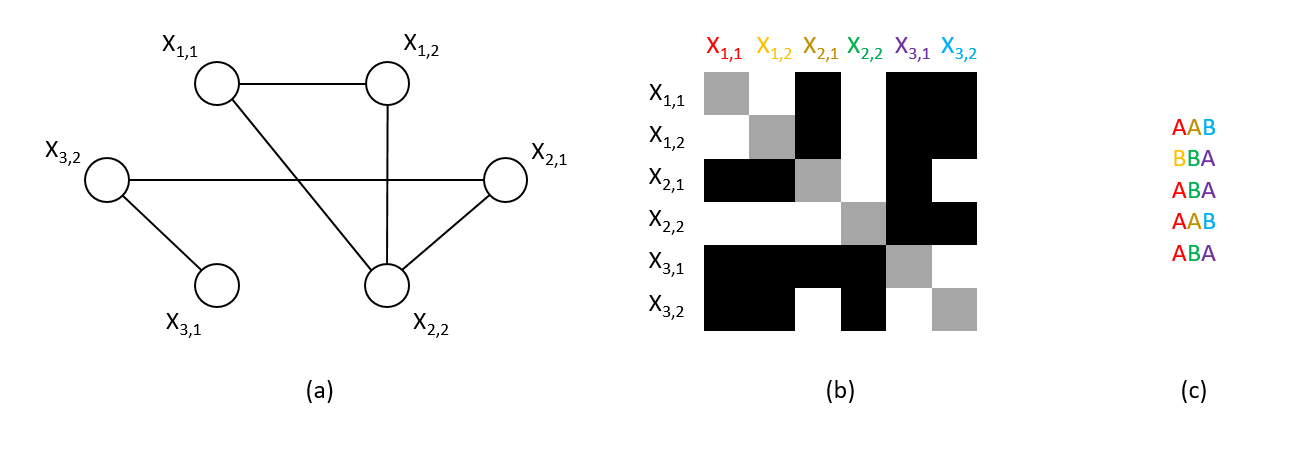
\includegraphics[width=\textwidth, keepaspectratio]{imgs/ggm.png}
                \caption{Illustration of a small system with only 3 sites and 2 amino acid types A and B:
                    (a) Gaussian graphical model representing the system.
                    (b) Sparsity pattern of the estimated inverse covariance matrix.
                    Cells associated to zero variables are drawn in black. (c) Corresponding MSA.}
                \label{thresholds}
            \end{center}
        \end{figure}

    \subsection{Inference}

        The solution chosen here is to estimate sparse inverse covariance matrices instead,
        by having recourse to Graphical Lasso algorithm~\cite{graphicalLasso}.
        The method assumes that observations follow a multivariate normal distribution
        characterized by the following probability density function:

        \begin{equation}
            f(x) = \frac{1}{\sqrt{(2\pi)^d \vert\Sigma\vert}} \exp{-\frac{1}{2} (x - \mu)^T \Sigma^{-1} (x - \mu)}
        \end{equation}

        where $d=21L$ is the number of components in vector $x$, $\mu$ is the theoretical mean and $\Sigma$ the theoretical covariance matrix.
        Let's express the log-likelihood of the data as a function of the inverse theoretical matrix $\Theta$:

        \begin{equation}
            \begin{split}
                \log{L}(\Theta) & = \sum\limits_{k=1}^{n} \log{f(x^{(k)})} \\
                & = \sum\limits_{k=1}^{n} \Bigg( -\frac{1}{2} (x^{(k)} - \mu)^T \Sigma^{-1} (x^{(k)} - \mu) - \log{\sqrt{(2\pi)^d \vert\Sigma\vert}} \Bigg) \\
                & = \sum\limits_{k=1}^{n} \Bigg( -\frac{1}{2} (x^{(k)} - \mu)^T \Theta (x^{(k)} - \mu) - \log{\sqrt{(2\pi)^d \frac{1}{\vert\Theta\vert}}} \Bigg) \\
                & = -\frac{1}{2} \sum\limits_{k=1}^{n} (x^{(k)} - \mu)^T \Theta (x^{(k)} - \mu)
                    - \frac{1}{2} \sum\limits_{k=1}^{n} \log{\Big((2\pi)^d \frac{1}{\vert\Theta\vert}\Big)} \\
                & = -\frac{n}{2} \trace\big(S \Theta\big) + \frac{n}{2} \log{\vert\Theta\vert} - \frac{1}{2} \sum\limits_{k=1}^{n} \log{(2\pi)^d} \\
            \end{split}
        \end{equation}

        The latter expression holds because the empirical mean $\bar{x}$ is equal to $\mu$ for any $\Sigma$.
        The objective function of Graphical Lasso is simply the log-likelihood penalized with $L_1$ norm.
        $L_1$ regularization is used instead of $L_2$ because
        of its non-asymptotic behaviour and therefore its ability to produce more zeroes among the parameter values.
        The solution to the optimization problem is described as:

        \begin{equation} \label{psicovobj}
            \begin{split}
                \hat{\Theta} & = \argmax_{\Theta} \ \ \log{L}(\Theta) - \rho' \norm{\Theta}_1 \\
                & = \argmax_{\Theta} \ \ -\frac{n}{2} \trace\big(S \Theta\big) + \frac{n}{2} \log{\vert\Theta\vert}
                    - \frac{1}{2} \sum\limits_{k=1}^{n} \log{(2\pi)^d} - \rho' \norm{\Theta}_1 \\
                & = \argmax_{\Theta} \ \ -\trace\big(S \Theta\big) + \log{\vert\Theta\vert} - \rho \norm{\Theta}_1 \\
            \end{split}
        \end{equation}

        The $L_1$ norm $\norm{\Theta}_1$ is the sum of absolute values of the elements in $\Theta$.
        $\rho$ is the regularization parameter and $\rho'$ is syntactic sugar for denoting the same
        parameter before division.

        In the second version of PSICOV, the objective function present in equation~\ref{psicovobj} is being
        optimized with the GLassoFast algorithm~\cite{sustik2012glassofast}, making the predictor more efficient
        than in its first version.

        The predicted contact map is finally obtained after applying the two following processing steps:
        \begin{itemize}
            \item The score $S_{ij}^{contact}$ between residues $i$ and $j$ is calculated as
                the $L_1$ norm of submatrix $\Theta_{ij}$:
            \item The average product correction introduced by Dunn et al.~\cite{dunn2007mutual}
                is applied to the resulting scores in order to better approximate the background
                mutual information between sites $i$ and $j$:
                \begin{equation}
                    PC_{ij} = S_{ij}^{contact} - \frac{\bar{S}_{i-}^{contact} \bar{S}_{-j}^{contact}}{\bar{S}^{contact}}
                \end{equation}
                Based on the formalism of the PSICOV study, $\bar{S}_{i-}^{contact}$ is the norm of row $i$ of $S^{contact}$
                for all columns except $i$, and $\bar{S}_{-j}^{contact}$ is the norm of column $j$ for all rows except $j$.
        \end{itemize}

        According to Sun et al.~\cite{sun2015predicting}, the solutions found by PSICOV may not be suitable for some proteins.
        Furthermore, the best solution could be far from the global optimum found by Graphical Lasso since the search space is huge.
        The suggested solution is to predict multiple contact maps and promote diversity among them by adding a new penalty term.

        \begin{equation}\label{mbest}
            \begin{split}
                & \min_{\Theta^{(m+1)}} \frac{1}{2} \trace\big(S \Theta\big) + \frac{1}{2}
                    \sum\limits_{k=1}^{n} \log{(2\pi)^d} - \frac{1}{2} \log{\vert\Theta\vert} \\
                & s.t. \ \ \ d(\Theta^{(k)}, \Theta^{(m+1)}) \ge \epsilon, \ \ k = 1, \dotsc, m
            \end{split}
        \end{equation}

        In that last equation, the distance constraint function $d$ is a convex and differentiable function defined as:

        \begin{equation}
            d(\Theta^{(k)}, \Theta) = - \sum\limits_{i, j} \delta_0(\theta^{(k)})_{i, j} \vert \Theta_{i, j} \vert
        \end{equation}

        where $\delta_0: \mathbb{R}^{21L \times 21L} \rightarrow \mathbb{R}^{L \times L}$ is such that
        $\delta_0(\Theta_{i, j})$ takes value $1$ if submatrix $\Theta_{i, j}$ is $0$, and $-1$ otherwise.
        The objective function is optimized using a second-order method and updating the solution in the Newton direction at each iteration.
        Finally, a contact map is obtained by selecting the submatrices among the solutions according to their sparsity.
        More specifically, submatrices are selected according to their nuclear norm, hence the sum of their singular values.
        The authors claim that nuclear norm is better than $L_1$ norm at taking into account the sparsity patterns of the
        different submatrices.

\section{Deep learning}

    \subsection{A definition of \textit{deep learning}}

        Behind the trendy words, it is quite difficult to find a consensus on the definition of \textit{deep learning}. According to many, the process of learning 
        deeply can only be achieved by deep neural networks. A deep articifical neural network is composed of a set of parameters and a large stack 
        (or graph) of mathematical operators designed to minimize an objective function.
        Each operation may be dependent on a subset of the network parameters.
        In most cases, the network can be described as a stack of operators. 
        The objective function is then a composition of all mathematical operations. Such a network is usually trained using the 
        backpropagation algorithm. The method consists in minimizing the objective function which is usually an average distance between what the network
        predicts on the basis of an input and what the human supervisor expects. More specifically, it is an iterative algorithm that evaluates the gradient of the 
        objective at each iteration and performs one step in the direction of the steepest descent in the parameter space. The algorithm is expected to stop
        once a global minimum has been reached.

        Deep learning is also often viewed as the capacity of a machine to create a hierarchical modelling of the data.
        This implies that the model can transform the data to high-level feature maps.
        According to Yoshua Bengio and Yann LeCun, neural networks only exemplify the notion of deep
        architectures. They provided a sufficiently good basis for a definition:

        \begin{quotation}
            Deep architectures are compositions of many layers of adaptive non-linear components,
            in other words, they are cascades of parameterized non-linear modules that contain
            trainable parameters at all levels. Deep architectures allow the representation of wide
            families of functions in a more compact form than shallow architectures, because they
            can trade space for time (or breadth for depth) while making the time-space product
            smaller, as discussed below. The outputs of the intermediate layers are akin to intermediate
            results on the way to computing the final output. Features produced by the lower
            layers represent lower-level abstractions, that are combined to form high-level features
            at the next layer, representing higher-level abstractions~\cite{40d5d7fd62cb44ba934a8a75d4b2b076}.
        \end{quotation}

        This definition seems to be suitable for stacked models: one can design a cascade of decision tree modules since decision trees are able to construct
        non-linear decision boundaries. The problem rather lies in determining if there exists a natural way to make them extract high-level features from data.
        Apart from that, the backpropagation algorithm for neural networks is going to be introduced in more details.

    \subsection{The backpropagation algorithm} \label{backpropagation}

        A description of backpropagation has to be made in order to understand how modern deep learning works. 
        Let's consider a feedforward neural network containing no cycle.
        Each of its layers can be viewed as a couple $(f_i(\theta_i, X), b_i(\theta_i, dX))$,
        where $f_i$ is the forward pass function (prediction function)
        of layer $i$, $b_i$ is the backward pass function, $\theta_i$ is the set of parameters,
        and $X, Y$ are input tensors of shapes compatible with $f_i$ and
        $g_i$, respectively, and $dX$ is the signal tensor propagated from next layer to current layer.
        Let's make the assumption that convolutional layers are two-dimensional and that input instances are image-like data.
        Also, let's consider a particular case of neural network consisting of a stack of neural layers instead of a graph:
        a feedforward neural network.
        Also, let $b$ be the number of instances in the input tensor (more commonly referred to as the batch size), 
        $w$ and $h$ respectively the width and height of the images, 
        and $c$ the number of channels. Finally, let $n$ be the number of layers and $m$ be the number of output neurons in the network.
        Knowing this, we are able to express the output $Y \in \mathbb{R}^{b \times m}$ of the network as such:

        \begin{equation}
            Y = (\bigcirc_{i=1}^{n} f_{\theta_i})(X)
        \end{equation}

        where $X \in \mathbb{R}^{b \times w \times h \times c}$ and $f_{\theta_i}(X)$ 
        is a more convenient notation for $f_i(\theta_i, X)$. We observe that the prediction
        function of the network is basically a large composition of functions.

        Such model is designed to optimize a function reflecting its ability to accurately predict a target value or to abstractly represent the input 
        data in a more general sense. Accordingly, let's introduce a generic loss function $L(Y): \mathbb{R}^{b \times m} \rightarrow \mathbb{R}$ that measures 
        the model's inability to fulfill the given task. Again, the loss function can be rewritten as a composition of the layer forward passes and the loss
        function, and the objective is to find the set of parameters that minimizes the loss function:

        \begin{equation}
            \hat{\theta} = \argmin_{\theta \in \Theta} \ell((\bigcirc_{i=1}^{n} f_{i, \theta_i})(X))
        \end{equation}

        where $\Theta$ is the set of all possible values for the parameter set $\theta = (\theta_1, \ldots, \theta_n)$.
        Since we are considering a loss function, the latter must be minimized. The generic task of minimizing a scalar continuous function can be achieved
        using numerous continuous optimization techniques  among gradient descent algorithms~\cite{DBLP:journals/corr/Ruder16}
        or quasi-Newton methods~\cite{LBFGS}. In practice, gradient descent approaches require more iterations to converge to a satisfying solution,
        but are much easier to implement. Also, contrary to quasi-Newton methods, they don't require to implicitly compute the hessian matrix of the loss
        function according to the network parameters, which makes them less computation-intensive. Let's consider the optimization of the loss function
        in the gradient descent framework. The loss function is minimized by moving in the parameter space in the direction of the loss gradient, with
        a step proportional to a parameter either determined empirically or adjusted during optimization phase, called learning rate.
        Luckily, since we are regarding our neural network as a stack of layers (viewed as nested functions), the gradient computation can be decomposed
        using the chain rule:

        \begin{equation} \label{eq:backprop}
            (f \circ g)'(X) = \nabla f(g(X)) \cdot g'(X)
        \end{equation}

        Knowing this, the gradient of $loss(\theta)$ according to the parameters $\theta_m$ of layer $m$ (for any layer $m$ with learnable parameters),
        can be decomposed as the following product:

        \begin{equation} \label{eq:loss}
            \nabla \ \ell(\theta_m) = \prod_{i=1}^m f'((\bigcirc_{p=1}^{i} f_{\theta_i})(X)) \cdot L'((\bigcirc_{j=1}^{n} f_{\theta_j})(X))
        \end{equation}

        \todo{Replace prime symbols by actual partial derivatives}

        Each factor $i$ of the product can be computed using the definition of function $f'_i$, and the current input to layer $i$.
        However, layer $i$ requires the factor from layer $i+1$ in order to compute loss gradient according to its own parameters.
        Consequently, the signal (the product of factors from layer $n$ to current layer $p$) is passed from layer $p+1$ to layer $p$.
        In a more general sense, the gradient signal is passed from the ouput layer to the input layer, hence the name "backpropagation".

        The move in the gradient direction with step $\alpha$ (the so-called learning rate) is such that:

        \begin{equation}
            \theta_k \leftarrow \theta_k - \alpha \cdot \nabla \ \mathbb{l}(\theta_k) \  \ \forall k \in \{1, \ldots, n\}
        \end{equation}

        This step is repeated until one of the stop criteria has been met. For example, the algorithm stops when a maximum number of iterations has been
        reached. However, gradient descent is not the only optimization algorithm that yields satisfying results in practice.
        For example, Limited-memory BFGS~\cite{LBFGS} relies on a second order approximation of the loss function given a limited number of past
        update vectors: this provides a better search direction but in return does not theoretically guarantee that the loss function actually decreases at each
        iteration.

    \subsection{Fully-connected layers}

        A \textit{Multi-layer perceptron} is a neural network composed of multiple layers,
        where each layer's forward pass consists of a linear combination
        followed by an element-wise non-linear activation function.
        Let $X^{(p)} \in \mathbb{R}^{n \times m}$ be the input matrix of layer $p$,
        $W \in \mathbb{R}^{m \times k}$ the weight matrix,
        $b \in \mathbb{R}^{k}$ the bias vector, $n^{(p)}$ the number of inputs to layer $p$
        and $\sigma$ the non-linear activation function of layer $p$.
        Each layer can than be formalized as follows:

        \begin{equation}
            X_{i, k}^{(p+1)} = \sigma \Big( \sum\limits_{j=1}^{n^{(k)}} X^{(p)}_{i, j} W_{j, k} + b_{k} \Big)
        \end{equation}

        Backpropagation requires to compute the partial derivatives of layer outputs with respect to current layer parameters:

        \begin{align}
            \frac{\partial X_{i, k}^{(p+1)}}{\partial W_{j, k}} & = \sigma' \Big( \sum\limits_{j=1}^{n^{(k)}} X_{i, j} W_{j, k} + b_{k} \Big) \ X_{i, j}^{(p)} \\
            \frac{\partial X_{i, k}^{(p+1)}}{\partial b_{k}} & = \sigma' \Big( \sum\limits_{j=1}^{n^{(k)}} X_{i, j} W_{j, k} + b_{k} \Big)
        \end{align}

        where $Y \in \mathbb{R}^2$ is the output matrix and $\sigma'(x)$ is the derivative of $\sigma(x)$,
        typically $\sigma(x) (1 - \sigma(x))$ for the sigmoid function.

        Multi-layer perceptrons have been proved to be Universal Approximators~\cite{hornik1991approximation},
        meaning that they can approximate feedforward prediction functions that minimize any training loss (loss function computed on the training set).
        However, this fact does not inform about the type of non-linear function to use in order to minimize
        a given loss function. More importantly, this does not guarantee that the model will perform well on unseen examples.
        Indeed, high representational power is required when the classification task is abstract.
        To overcome this problem and lower the validation loss as much as possible, data scientists usually stack more layers on top of each other,
        but this may imply high computational requirements. Convolutional layers are used instead of dense weight matrices.

    \subsection{Convolutional layers} \label{convlayers}

        One of the major advances in semantic segmentation
        is due to Convolutional Neural Networks (CNNs)~\cite{DBLP:journals/corr/Garcia-GarciaOO17}.
        A CNN is an artificial neural network made of a stack of neural layers~\cite{lecun1998gradient}. One characteristic of CNNs is the
        presence of convolutional filters that map raw data to more abstract features. Each filter (or kernel) is locally connected to its output unit, which
        allows the convolutional layer to capture some local information about the inputs, as opposed to fully-connected layers that don't take any spatial
        information into account when passing data forward. This procedure is inspired by the notion of receptive field introduced 
        by Hubel and Wiesel~\cite{Hubel1962}.

        Weights are no longer stored in a bidimensional matrix since all inputs are no longer connected to each neuron of the current layer.
        Instead, each neuron is connected to a certain neighborhood of inputs. In this way, the network drastically reduces its number of parameters
        but still takes the spatial dependence of the data into account. If the convolutional layer is designed for processing multi-channel images for example,
        the parameters will be stored in a 4-dimensional tensor. Let $W \in \mathbb{R}^{b \times h \times w \times n_c}$ be the weights of the convolutional filters,
        $X^{(p)} \in \mathbb{R}^{b \times h_b \times w_b \times n_c}$ the input images of layer $p$, $b \in \mathbb{R}$ the bias vector
        and $X^{(p+1)} \in \mathbb{R}^{b \times (\floor{(h_b - h) / \beta_1} + 1) \times (\floor{(w_b - w) / \beta_2} + 1) \times n_f}$
        the output feature maps. Let's consider the relation between the input images and the output feature maps:

        \begin{equation} \label{eq:conv2D}
            X_{i, j, k, l}^{(p+1)} = \sigma \Big( \sum\limits_{\alpha=1}^h \sum\limits_{\delta=1}^w
                \sum\limits_{c=1}^{n_c} W_{j, \alpha, \delta, c} X_{i, k+\beta_1 \alpha, l+\beta_2 \delta, c}^{(p)} + b_{j} \Big) 
        \end{equation}

            where $i$ is the image identifier, $j$ is the filter index, $n_c$ is the number of channels, $h$ is the filter height, $w$ is the filter width
            and $(\beta_1, \beta_2)$ are the strides (vertical and horizontal distances between neighboring pixels in the neighborhood connected to a same neuron).
            Partial derivatives are simply given by:

        \begin{align}
            \frac{\partial X_{i, j, k, l}^{(p+1)}}{\partial W_{j, \alpha, \delta, c}} & = 
                \sigma' \Big( \sum\limits_{\alpha=1}^h \sum\limits_{\delta=1}^w \sum\limits_{c=1}^{n_c} W_{j, \alpha, \delta, c}
                X_{i, k+\beta_1 \alpha, l+\beta_2 \delta, c}^{(p)} + b_{j} \Big) X_{i, k+\beta_1 \alpha, l+\beta_2 \delta, c} \\
            \frac{\partial Y_{i, j, k, l}}{\partial b_{j}} & =
                \sigma' \Big( \sum\limits_{\alpha=1}^h \sum\limits_{\delta=1}^w \sum\limits_{c=1}^{n_c} W_{j, \alpha, \delta, c}
                X_{i, k+\beta_1 \alpha, l+\beta_2 \delta, c}^{(p)} + b_{j} \Big)
        \end{align}

        Just as in the case of fully-connected layers, the computations for the signal propagation are not shown because this report is intended to remain brief.
        Contrary to neural networks, it must be noted that random forest implementations are rarely equipped with convolutional filters or even multivariate 
        splits. Even in computer vision applications, univariate decision trees are the most frequently used trees in ensemble learners.

        \todo{Double check indices and whether symbols have been correctly defined}

    \subsection{Activation functions}

        An activation function describes the output value of a neuron and is biologically inspired. It is a mathematical representation
        of the level of action potential sent along its axon. More formally, it is a non-linear scalar function that takes a scalar as input.
        The presence of activation functions in neural networks along with fully-connected layers allows them to increase their representational
        power. Indeed, a stack of fully-connected layers without activation functions would have the same representational power as a single
        fully-connected layers, since a linear combination of linear combinations is itself a linear combination. Thus, activation functions
        help to actually build a hierarchical representational of the data by folding the hyperplane containing the data points multiple times
        and at each layer.

        However, not every activation function is suitable for backpropagation and one of the reasons for the success of deep learning is the low
        computation requirements for the gradients. Most of the activation functions are non-prametric and element-wise, which makes it easy
        to compute the signal during backward pass.

        The best known activation function is the sigmoid function $\sigma(x)$.
        It has the property to have a derivative $\sigma'(x)$ expressed as a function of $\sigma(x)$,
        which speeds up computation times, assuming that the neural outputs are cached.

        \begin{equation}
            \begin{split}
                \sigma(x) & = \frac{1}{1 + \smallexp{-x}} = \frac{\smallexp{x}}{1 + \smallexp{x}} \\
                \sigma'(x) & = \sigma(x) (1 - \sigma(x))
            \end{split}
        \end{equation}

        However, LeCun~\cite{efficientBackprop} does not recommend standard sigmoid functions because normalizing
        activation functions generally ensure better performance.
        For this reason, the hyperbolic tangent is suitable because its outputs are centered around zero. 
        Also, its derivative $\tanh'(x)$ is expressed as a function of $\tanh(x)$ which is computationally convenient.
        Finally, an additional linear term can be added in order to
        avoid flat areas, leading to an activation function of the following form: $f(x) = \tanh(x) + ax$.

        \begin{equation}
            \begin{split}
                \tanh(x) & = \frac{\smallexp{x} - \smallexp{-x}}{\smallexp{x} + \smallexp{-x}} = \frac{\smallexp{2x} - 1}{\smallexp{2x} + 1} \\
                \tanh'(x) & = 1 - \tanh^2(x)
            \end{split}
        \end{equation}

        Assuming that target values are in the set $\{-1, 1\}$ in the framework of binary classficaition,
        the hyperbolic tangent can be linearly modified to obtain a new function of the form $f(x) = 1.7159 \tanh(\frac{2}{3} x)$.
        Such an activation function is profitable because, has its second derivative maximized at $x = -1$ and $x = 1$, avoiding
        saturation effects.

        The chain rule informs us that the gradient of a given layer is factorized as a product of vectors/matrices computed by previous layers.
        Because the norm of gradients w.r.t. activation functions is always less than one for both tanh and standard sigmoid,
        deep architectures are often subject to vanishing gradients. Linear rectifier units (ReLU) are piecewise linear functions designed to solve
        these issues by keeping positive inputs unchanged. Let's note that ReLU is not differentiable at $x = 0$ but inputs are rarely zero in practice.

        \begin{equation}
            \begin{split}
                \text{ReLU}(x) & = \max{(x, 0)} \\
                \text{ReLU}'(x) & = 
                \begin{cases}
                    1 & \text{if } x > 0 \\
                    0 & \text{if } x < 0
                \end{cases}
            \end{split}
        \end{equation}

        The outputs of a neural network are often desired to sum to one, especially when the classification task is to assign each class to a probability
        conditionally to the network's input. In the case where there are $m$ classes, the output layer is composed of $m$ neurons where the activation
        function associated to neuron $i$ is given by:

        \begin{equation}
            \begin{split}
                \sigma(x^{(i)}) & = \frac{\smallexp{x^{(i)}}}{\sum\limits_{k=1}^m \smallexp{x^{(k)}}} \\
                \sigma'(x^{(i)}) & = \sigma(x^{(i)}) (1 - \sigma(x^{(i)}))
            \end{split}
        \end{equation}

        where $x^{(i)}$ is the component $i$ of the output vector.
        This function is identical to the Boltzmann distribution introduced in section \ref{potts}.


    \subsection{Batch normalization} \label{batchnorm}

        According to Ioffe and Szegedy~\cite{DBLP:journals/corr/IoffeS15}, deep neural networks are subject to a phenomenon
        called \textbf{internal covariate shift}. When the learning rate is too large, the distribution of a layer's outputs
        is drastically altered, making it difficult to train the next layer since the latter is constantly adapting to the new
        distribution. Batch normalization helps dealing with this issue and allows us to run the training algorithm with less
        careful parameter initialization and larger learning rate.

        When the network is training with batch learning, its parameters are updated every batch. Therefore, the distribution
        of each layer's outputs is changed at each batch. This is the reason for using the statistics of each batch individually
        to normalize the data between layers.

        \begin{table}[H]
            \centering
            \begin{tabular}{|l|c|c|}
                \hline
                Name & Number of samples involved & Formula \\
                \hline
                \hline
                Average (true) gradient & $N$ & $\frac{1}{N} \sum\limits_{i=1}^N \nabla L(f_{\theta}(X_i))$ \\
                \hline
                Batch gradient & $\vert B \vert$ & $\frac{1}{\vert B \vert} \sum\limits_{i \in B} \nabla L(f_{\theta}(X_i))$ \\
                \hline
                Sample gradient & $1$ & $\nabla L(f_{\theta}(x))$ \\
                \hline
            \end{tabular}
            \captionof{table}{Types of gradients and gradient approximations used in common optimization methods.}
            \label{gradients}
        \end{table}

        \todo{Backpropagating sample gradients in fully-convolution networks}

        \begin{equation}
            \begin{split}
                \mu_{\mathcal{B}} & = \frac{1}{\vert\mathcal{B}\vert} \sum\limits_{i=1}^{\vert\mathcal{B}\vert} x_i \\
                \sigma_{\mathcal{B}}^2 & = \frac{1}{\vert\mathcal{B}\vert} \sum\limits_{i=1}^{\vert\mathcal{B}\vert} (x_i - \mu_{\mathcal{B}}^2) \\
                \hat{x}_i & \leftarrow \gamma \frac{x_i - \mu_{\mathcal{B}}}{\sqrt{\sigma_{\mathcal{B}}^2 + \epsilon}} + \beta
            \end{split}
        \end{equation}

        Optimize $\beta, \gamma$ with backpropagation. \todo{}

    \subsection{Regularization}

	From an optimization perspective, regularization is a penalty used to prevent 
	parameters from growing arbitrarily big during training.
	According to Occam's law of parsimony, simpler hypotheses should be privileged over more complex ones.
	Therefore, when the neural architecture involves a large number of free parameters
	in the presence of relatively few data samples,
	regularization helps reducing parameters importance and converging to less arbitrary parameter values.
	From a Bayesian perspective, regularization provides a prior distribution over the model parameters.
	In Bayes formula, the posterior $P(\theta \vert X, \alpha)$ is a function of both the prior
	$P(\theta \vert \alpha)$ and the likelihood of the data $P(X \vert \theta, \alpha)$ under model $\theta$.

	\begin{equation}
	    P(\theta \vert X, \alpha) = \frac{P(X \vert \theta, \alpha)\,P(\theta \vert \alpha)}{P(X \vert \alpha}
	\end{equation}

	The relation between the loss function of a neural network and Bayes formula can be established
	by proving the two following points:

	\begin{itemize}
	    \item The log-likelihood of the data is equal to the negative cross-entropy.
	    \item The regularization term is proportional to the prior distribution of the parameters.
	\end{itemize}

	The first part is easy to show since negative log-likelihood can be obtained from binary cross-entropy:
	\begin{align}
		CE(\hat{y}, y) & = - \log{\prod\limits_{i=0}^n P(\hat{y_i})^{y_i}}  \\
		& = -\sum\limits_{i=0}^n y_i \log{\hat{y}} + (1 - y_i) \log{1 - \hat{y}}
	\end{align}
	This allows us to provide a statistical interpretation of the loss function.
	Regarding priors, L1 and L2 regularizations are going to be introduced in the following two sections.

	\subsubsection{L1 regularization}

	   Adding a L1 regularization term to the loss function reduces to providing a Laplacian
	   prior on model parameters.  

	   \begin{align}
	       \max_{\theta}\, \log{P(\theta \vert \eta, b)} 
		   & = \max_{\theta}\, \log{\prod\limits_{i=1}^m \, \frac{1}{2b_i}\,
		   \exp{\frac{- \abs{\theta_i - \eta_i}}{b_i}}} \\
		   & = \max_{\theta}\, \sum\limits_{i=1}^m \frac{- \abs{\theta_i - \eta_i}}{b_i} - \log{2b_i} \\
		   & = \min_{\theta}\, \sum\limits_{i=1}^m \abs{\theta_i - \eta_i}
	   \end{align}

	   By setting vector $\eta \in \mathbb{R}^m$ to $0$, the resulting regularization term
	   takes its final well-known form $\sum\limits_{i=1}^m \abs{\theta_i}$.

	\subsubsection{L2 regularization}
		   
	   L2 regularization acts as a Gaussian prior on model parameters.
	   This can be highlighted by setting the probability density function of the Gaussian
	   distribution as the prior and show that the regularization term is proportional
	   to the logarithm of the product of priors.

	   \begin{align}
               \max_{\theta}\, \log{P(\theta \vert \eta, \sigma)}
		   & = \max_{\theta}\, \log{\prod\limits_{i=1}^m \, \frac{1}{\sqrt{2\pi\sigma^2}} 
		   \exp{-\frac{(\theta - \eta)^2}{2\sigma^2}}} \\
		   & = \max_{\theta}\, \sum\limits_{i=1}^m \, -\frac{(\theta_i - \eta_i)^2}{2\sigma^2}
		   - \log{\sqrt{2\pi\sigma^2}} \\
		   & = \min_{\theta}\, \sum\limits_{i=1}^m \, (\theta_i - \eta_i)^2 
           \end{align}

	   Again, by setting vector $\eta \in \mathbb{R}^m$ to $0$, the regularization term takes its
	   final form $\sum\limits_{i=1}^m \theta_i^2$.

    \subsection{Optimization algorithms}

        The gradient vector is obtained by concatenating the gradients w.r.t.
	each layer's parameter vector. This final gradient vector
        gives an improvement direction, but a decrease of the loss function
	is guaranteed by moving by a arbitrary small step in the parameter space.

        \todo{Overview: \cite{DBLP:journals/corr/Ruder16}}

        \todo{Adam: \cite{DBLP:journals/corr/KingmaB14}}

        \todo{Adadelta: \cite{DBLP:journals/corr/abs-1212-5701}}

        \todo{L-BFGS: \cite{LBFGS}}

\subsection{Input features} \label{inputfeatures}

    \subsubsection{Global features}

        \paragraph{Protein length}

      	    Protein length is computed as the number of residues in the protein sequence.
    	    It provides complementary information that convolutional layers cannot capture.
     	    Indeed, fully-connected neural networks have the ability to handle arbitrary-sized
    	    features maps at the cost of not knowing the dimensionality of their inputs.
    	    Injecting protein length as a supplementary global feature may help the model
    	    to infer the maximum distance in long-range contacts.

	   \paragraph{Effective number of sequences} \label{meff}

    	    The number of effective sequences is equal, w.r.t. to a given threshold,
    	    to the number of non-redundant sequences in the set of homologous sequences.
    	    It provides a bound on the potential performance of the DCA methods involved
    	    in the pipeline.

            \begin{equation}
                M_{eff} = \sum_{i=1}^m w_i = \sum_{i=1}^m \frac{1}{|\{r(s_i, s_j) \ge \tau \quad \forall j \in \{1, \dotsc, m\}\}|}
            \end{equation}

            $w_i$ is the weight associated to homologous sequence $i$.
            $r(s_i, s_j)$ is the identity rate between sequences $s_i$ and $s_j$, in other words
            the number of matching residues (including gaps) divided by the total number of positions,
            which is assumed to be equal in both sequences.

    \subsubsection{1-dimensional features}

        \paragraph{One-hot encoded sequence}

            Given an amino acid sequence $\{s_1, s_2, \ldots,
            s_L\}$ of size L, the one-hot encoded sequence
            is a matrix $X \in \{0, 1\}^{L \times 21}$
            where $x_{ia}$ is one if $s_i = a$ and zero otherwise.

        \paragraph{Solvent accessibility prediction}

            Solvent accessibility or solvent-accessible surface is the surface of
            a molecule that is accessible to a solvent. Such feature contains indirect
            information about the protein structure since residues with low accessibility
            are more likely to be internal to the protein and vice versa.
            When atomic coordinates are available, solvent accessibility can be computed exactly
            using the rolling ball algorithm from Shrake and Rupley~\cite{shrake1973environment},
            as illustrated by figure~\ref{rollingball}.
            Since protein structure is not available for target proteins of the test set,
            supervised models rely on predicted solvent accessibility instead.

            \begin{figure}[H]
                \begin{center}
                    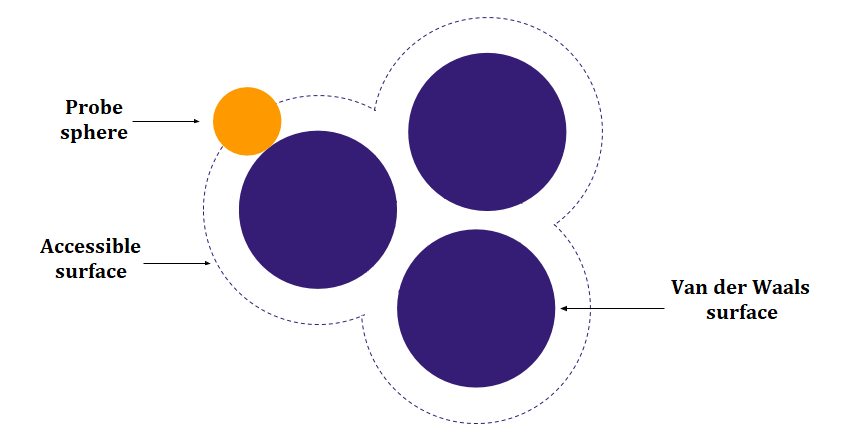
\includegraphics[height=5cm, keepaspectratio]{imgs/accessibility.png}
                    \caption{Accessible surface, obtained by "rolling" a probe sphere (a molecule
                        of solvent, colored in orange) on the Van der Waals surface of a biomolecule
                        (colored in blue).}
                    \label{rollingball}
                \end{center}
            \end{figure}

            The RaptorX-Property server~\cite{wang2016raptorx} is publicly available and provides
            predictions for relative solvent accessibility (RSA). The latter is defined as the predicted
            accessible surface of a residue divided by the maximum possible solvent accessibility
            for that amino acid, which is more convenient more machine learning since it does not a
            normalization step. RSA prediction is 3-state. A residue can be either:
            \begin{itemize}
                \item Buried (B), when RSA is below 10\%.
                \item Intermediate (I), when RSA is between 10\% and 40\%.
                \item Exposed (E), when RSA is above 40\%.
            \end{itemize}


        \paragraph{Predicted secondary structure prediction}

            As defined by DSSP, there are 8 different states for encoding
            secondary structure: H (alpha-helix),
            G (310 helix), I (pi-helix), E (beta-strand), B (beta-bridge),
            T (beta-turn), S (high curvature loop) and L (irregular loop).
            In practice, secondary structure prediction is either 3-state
            or 8-state~\cite{wang2016raptorx}.
            \begin{itemize}
                \item \textbf{Alpha-helix} is the most common pattern among
                    secondary structures.
                \item \textbf{310 helix}:  TODO
                \item \textbf{Pi-helix}: TODO
                \item \textbf{Beta-strand}: TODO
                \item \textbf{Beta-bridge}: TODO
                \item \textbf{Beta-turn}: TODO
                \item \textbf{High curvature loop}: TODO
                \item \textbf{Irregular loop}: TODO
            \end{itemize}

            When the number of labels is limited to three,
            the predictor only focuses on beta-strands (E), alpha-helices (H)
            and a third state which is the union of the six remaining states (C).
            Formally, a $m$-state secondary structure prediction is a matrix
            $S \in [0, 1]^{L \times m}$ where element $S_{i,j}$ is the probability
            of residue $i$ being in conformation $j$,
            with each row summing to one.

        \paragraph{Region disorder prediction}

            Region disorder prediction is a vector $D \in [0, 1]^L$
            where $D_i$ is the probability of residue $i$ being in a region
            of missing residues in the X-ray 3D structure. Residues with high
            probability are said to be disordered.
            Such features are also made publicly available by the 
            RaptorX-Property server~\cite{wang2016raptorx}.

        \paragraph{Amino acid frequencies}

            Amino acid frequencies are position-specific features that can be efficiently computed.
            Let $S \in \{0, \ldots, \naatypes\}^{M \times L}$ be a
            MSA matrix containing $M$ sequences aligned to a target
            sequence of length $L$. Then amino acid frequencies can be arranged
            in a matrix $F \in \mathbb{R}^{L \times \naatypes}$
            where element $F_{ia}$ is computed as follows:

            \begin{equation}
                F_{ia} = \frac{1}{M} \sum\limits_{k=1}^M \delta(S_{ki}, a)
            \end{equation}

        \paragraph{Position-Specific Scoring Matrix}

            \todo{PSI-PRED: \cite{jones1999protein}}

        \paragraph{Atchley factors}

            \todo{Atchley: \cite{Atchley2005}}

        \paragraph{Self-information}

            In information theory, self-information is the amount of information, in bits,
            obtained by observing a random variable. In particular, let $x_{ij} \in \{0, 1\}$ be
            a binary variable indicating the presence of an amino acid of type $j$ at site $i$.
            The self-information suggested by Michel et al~\cite{Michel383133} can be formalized
            with the following equation:

            \begin{equation}
                I_{ij} = \log_2 (p_{ij} / \langle p_i \rangle)
            \end{equation}

            where $p_{ij}$ is the probability of observing amino acid $j$ at site $i$ among all residues
            of given MSA, and $\langle p_j \rangle$ is the frequency of amino acid $j$
            in the Uniref50 dataset.

        \paragraph{Partial entropies}

            \todo{ \cite{Michel383133}}

            \begin{equation}
                S_i = p_i \log_2 (p_i / \langle p_i \rangle)
            \end{equation}

    \subsubsection{2-dimensional features}

        \paragraph{Mutual Information and Normalized Mutual Information}

            Following the formalism described in \cite{Michel383133}, MI is described as:

            \begin{equation}
                MI(x, y) = \sum\limits_{x, y} P(x, y) \log \Big( \frac{P(x, y)}{P(x) \cdot P(y)} \Big)
            \end{equation}

            \begin{equation}
                NMI(x, y) = \frac{MI(x, y)}{\sqrt{S(x) \cdot S(y)}}
            \end{equation}

            Average product correction is applied to both MI and NMI.

        \paragraph{Cross-entropy}

            Cross-entropy is computed in \cite{Michel383133} using the following formula:

            \begin{equation}
                H(x, y) = S(x) + S(y) - MI(x, y)
            \end{equation}

        \paragraph{Contact potential}

            \todo{}

        \paragraph{Evolutionary couplings}

            Predictions from GaussDCA, plmDCA or PSICOV can be used as input to the deep
            learning approach. Only top predicted contacts are informative, TODO

        \paragraph{Covariance}

            Covariance matrices are computed as in equation \ref{covariance} of the section
            about Gaussian graphical models (see section \ref{graphicalmodels}).
            In PSICOV~\cite{doi:10.1093/bioinformatics/btr638}, the inferred covariance
            matrix is averaged across the dimension of amino acid types.
            In DeepCov~\cite{doi:10.1093/bioinformatics/bty341}, the full matrix is used
            as input to the supervised model.

    \subsection{Features for the proposed approach}

        The lines which will follow are a discussion about the features to use as inputs
        to the model. At the outset, it should be noted that all models rely on
        two-dimensional features. Those features are either predictions from another
        predictor, covariance matrices or correlated mutations.
        However, using intermediary predictions requires installing additional software.
        PSICOV is written in C and can be recompiled. The official implementation of
        plmDCA was originally made in Matlab, forcing researchers to add a whole raft
        of external tools. plmDCA, as well as GaussDCA now have a Julia implementation,
        making them more accessible. The proposed approach incorporates all three
        predictors in its pipeline.

        \begin{landscape}
            \begin{table}[H]
                \centering
                \begin{tabular}{llcccccc}
                    \hline
                    Features & & DeepCov & DeepContact & PConsC4 & DNCON2 & RaptorX & Proposed method \\
                    \hline
                    \hline
                    Global & Protein length & & & & $\times$ & & $\times$ \\
                    & Meff & & & & $\times$ & & $\times$ \\
                    \hline
                    1-dimensional & Column log-entropy & & $\times$ & & & & \\
                    & Predictors stdv & & $\times$ & & & & \\
                    & Encoded sequence & & & $\times$ & & & $\times$ \\
                    & \textbf{Solvent accessibility} & & $\times$ & & $\times$ & $\times$ & $\times$ \\
                    & \textbf{Predicted SS} & & $\times$ & & $\times$ & $\times$ & $\times$ \\
                    & AA frequencies & & $\times$ & $\times$ & & & \\
                    & PSSM & & & & $\times$ & $\times$ & \\
                    & Atchley factors & & & & $\times$ & & \\
                    & Self-information & & & $\times$ & & & $\times$ \\
                    & Partial entropies & & & $\times$ & & & $\times$ \\
                    \hline
                    2-dimensional & Mutual Information (MI) & & & $\times$ & $\times$ & $\times$ & $\times$ \\
                    & Normalized MI & & $\times$ & $\times$ & $\times$ & & $\times$ \\
                    & Cross-entropy & & $\times$ & $\times$ & & & $\times$ \\
                    & \textbf{Contact potential} & & & & & $\times$ & \\
                    & \textbf{EVFold} & & $\times$ & & & & \\
                    & \textbf{CCMPred} & & $\times$ & & $\times$ & $\times$ & \\
                    & \textbf{plmDCA} & & & & $\times$ & & \\
                    & \textbf{GaussDCA} & & & $\times$ & & & $\times$ \\
                    & \textbf{PSICOV} & & & & & & \\
                    & Covariance & $\times$ & & & & & \\
                    \hline
                \end{tabular}
                    \caption{Features used in state-of-the-art deep learning approaches.
                        Feature extraction methods that rely on external tools (excluding
                        MSA tools) are highlighted in bold.}
                    \label{features}
            \end{table}
        \end{landscape}
\section{Deep learning and PCP}


    \todo{DNCON2: \cite{doi:10.1093/bioinformatics/bty341}}

    \todo{PConsC4: \cite{Michel383133}, zero-padding, based on U-net: \cite{DBLP:journals/corr/RonnebergerFB15}}

    \todo{DeepContact: \cite{DeepContact}}

    \todo{RaptorX-Contact: \cite{RaptorX}, zero-padding}

    \todo{DeepCov: \cite{doi:10.1093/bioinformatics/bty341}}

    \todo{TiramiProt: \cite{TsardakasRenhuldt1228846}}

    \todo{\cite{DeepConPred2}}

    \todo{proteinloopmodeling}

    Benchmark with both accuracy and standard deviation w.r.t. proteins.


    \todo{Deep architectures in PCP: \cite{di2012deep}}

    \todo{ResNet: \cite{DBLP:journals/corr/HeZRS15}}
    \todo{DenseNet: \cite{huang2017densely}}
\chapter{Materials and methods}

\section{Datasets}

  Five datasets have been used in the framework of this thesis:
  one for training the model, one for optimizing the hyper-parameters, and three for benchmarking.
  The training set is a set of 354 proteins including the 150 families reported in the original PSICOV
  paper~\cite{doi:10.1093/bioinformatics/btr638}, plus a subset of the first benchmark set used by
  Michel et al. to evaluate PConsC3~\cite{Skwark079673}.
  The validation set is composed of the 30 protein families from the validation set of PConsC3,
  which itself is a subset of the test set of PConsC2~\cite{10.1371/journal.pcbi.1003889}.

  Three test sets have also been considered in order to make a direct comparison with the state-of-the-art RaptorX-Contact predictor.
  The first test set embodies the 105 protein domains from the CASP11 experiment, the second test set 76 proteins from the CAMEO
  project, and the fourth test set 398 membrane proteins.

  \subsection{Homology reduction}

    A straightforward method for reducing homology between two set of proteins is to
    remove proteins that have a sequence identity rate above a given threshold.
    As a rule of thumb, this threshold is usually set to 40\%.
    Identity rates were computed by running Needleman-Wunsch algorithm on each
    pair of proteins coming from two different datasets. Score matrix was set
    such that exact matches give a score of 1 and any mismatch gives a penalty of -1.
    Indeed this approach promotes global alignments with maximum identity rates.

    \begin{table}[H]
      \centering
      \begin{tabular}{|l|c|c|c|}
        \hline
        Identity rate & Minimum & Average & Maximum \\
        \hline
        \hline
        Training set - CASP11 & 5.4 & 22.4 & 32.5 \\
        PSICOV150 - CASP11 & 7.3 & 22.9 & 39.7 \\
        PSICOV150 - CAMEO & 6.2 & 21.7 & 34.4 \\
        Training set - CAMEO & 4.0 & 21.3 & 32.5 \\
        PSICOV150 - Membrane & 7.6 & 22.2 & 74.0 \\
        \hline
      \end{tabular}
      \captionof{table}{Identity rates between training and benchmark sets, expressed as percentages.}
      \label{identityrates}
    \end{table}

    Similarity rates are more informative than identity rates because amino acids
    are very likely to mutate across evolution towards amino acids that share
    similar physico-chemical properties, and such measures take these mutations
    into account. However, ECOD H-classes~\cite{10.1371/journal.pcbi.1003926}
    were used instead of similarity rates because they can potentially give more
    evidence on whether two sequences are evolutionary related.
    Therefore, proteins belonging to different datasets and sharing the same
    ECOD H-class have been rejected.

    \todo{Computation of identity rates, Common ECOD H-classes}

    \begin{figure}[H]
      \begin{center}
        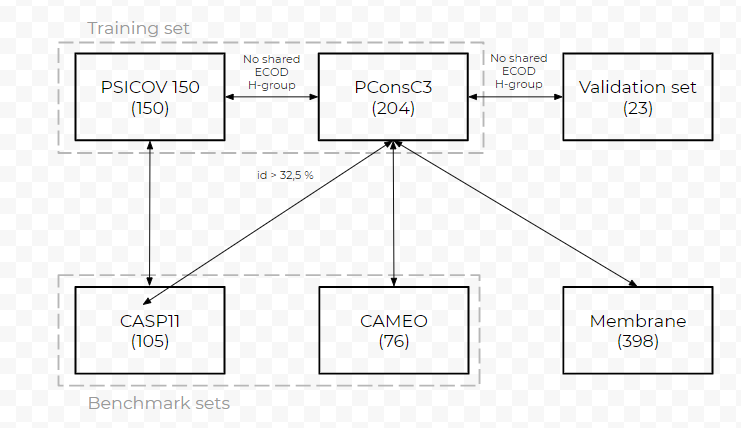
\includegraphics[width=\textwidth, keepaspectratio]{imgs/datasets.png}
         \caption{Homology reduction between the different datasets}
        \label{homology_reduction}
      \end{center}
    \end{figure}

  \subsection{PSICOV Dataset}

    The PSICOV~\cite{doi:10.1093/bioinformatics/btr638} dataset is composed of 150 families
    and associated multiple sequence alignments
    taken from the Pfam database, each containing more than 1000 homologous sequences
    and a target sequence with high-resolution ($\le$ 1.9 \AA{}) X-ray crystallographic structure.
    Each target sequence contains exactly one copy of the Pfam domain, has a length lower than
    275 and greater than 50 residues. The number of unique sequences in each multiple sequence
    alignment strongly varies from one family to another.
    AraC-like ligand binding domain (implied in DNA-binding transcription and
    sequence-specific DNA binding) accounts for 511 unique sequences, compared to 74 836 sequences
    for the response regulator receiver domain.

  \subsection{CASP11}

    CASP10~\cite{doi:10.1002/prot.24452}
    CASP11~\cite{doi:10.1002/prot.25064}


    \todo{}

  \subsection{CAMEO}

    CAMEO~\cite{haas2013protein}

    \todo{}

  \subsection{Membrane proteins}

    \todo{}

  \subsection{Feature extraction}

    \todo{Profile HMMs: \cite{eddy1998profile}}
    MSAs have been created using HHblits~\cite{HHblits} (version as of the date of 26th February 2016) on the Uniprot20 database
    with an e-value of 1. Parameters have been set in such a way that all sequences in each of the database MSAs are aligned.
    The obtained MSAs have been used as input to all other predictors and intermediate predictors, allowing for easier comparability.

    All protein sequences, structures, MSAs and intermediate predictions used in this thesis come from the datasets that were publicly
    available at the address \url{http://pconsc3.bioinfo.se/pred/download/} as on the date of 28th December 2018.
    Information available in these datasets is the following:

    \todo{PDB parser to obtain distance and contact maps}

    \begin{itemize}
      \item Protein sequence in FASTA format
      \item \index{MSA} obtained using HHblits on the corresponding protein family
      \item Atom 3D coordinates
      \item PhyCMAP~\cite{PhyCMap} intermediate predictions
      \item plmDCA~\cite{EKEBERG2014341} intermediate predictions
      \item GaussDCA~\cite{10.1371/journal.pone.0092721} intermediate predictions
      \item Predictions made by PConsC3~\cite{Skwark079673} at each layer of the model
      \item CCMPred~\cite{CCMPred} predictions (only available in the 4 test sets)
      \item EVFold~\cite{Sheridan021022} predictions (only available in the 4 test sets)
      \item PSICOV~\cite{doi:10.1093/bioinformatics/btr638} predictions (only available in the 4 test sets)
      \item MetaPSICOV~\cite{MetaPSICOV} predictions (only available in the 4 test sets)
    \end{itemize}

    \todo{Took alignments from PConsC2 and PConsC3 -> model not influenced by the new releases of alignments tools}
    \todo{What about the protein structures?}

    \todo{Oversampling negative class: \cite{markowski2016oversampling}}

\section{Summary of input features}

  As described in section \ref{inputfeatures}, input features can be split into three categories:
  global, 1-dimensional and 2-dimensional features.
  The proposed model takes as input the protein length, the effective number of sequences
  in the corresponding MSA, position-specific statistics,
  residue pair-specific statistics, and predictions made by PSICOV, plmDCA and GaussDCA.
  Additionaly to these features, secondary structure, solvent accessibility and
  region disorder are predicted by RaptorX-property server and added to the rest of
  1-dimensional features.
  \todo{cite RaptorX-property}

  \begin{table}[H]
    \centering
    \begin{tabular}{|l|l|c|}
      \hline
      Category & Feature name & Dimensionality \\
      \hline
      \hline
      Global & Protein length $L$ & scalar \\
             & Effective number of sequences $M_{eff}$ & scalar \\
      \hline
      1-dimensional & One-hot-encoded sequence & $L \times \naatypes$ \\
                    & Self-information & $L \times \naatypes$ \\
                    & Partial entropy & $L \times 2 \cdot \naatypes$ \\
                    & Predicted secondary structure & $L \times 3$ \\
                    & Solvent accessibility & $L \times 3$ \\
                    & Region disorder & $L$ \\
      \hline
      2-dimensional & Mutual information & $L \times L$ \\
                    & Normalized mutual information & $L \times L$ \\
                    & Cross-entropy & $L \times L$ \\
                    & PSICOV predictions & $L \times L$ \\
                    & GaussDCA predictions & $L \times L$ \\
                    & plmDCA predictions & $L \times L$ \\
      \hline
    \end{tabular}
    \captionof{table}{Input features of the proposed model.
      Global features are scalar values, whereas dimensional
      features are presented in the form of matrices of given shape.}
    \label{hyperparams}
  \end{table}

\section{Proposed architecture}

  \begin{figure}[H]
    \begin{center}
      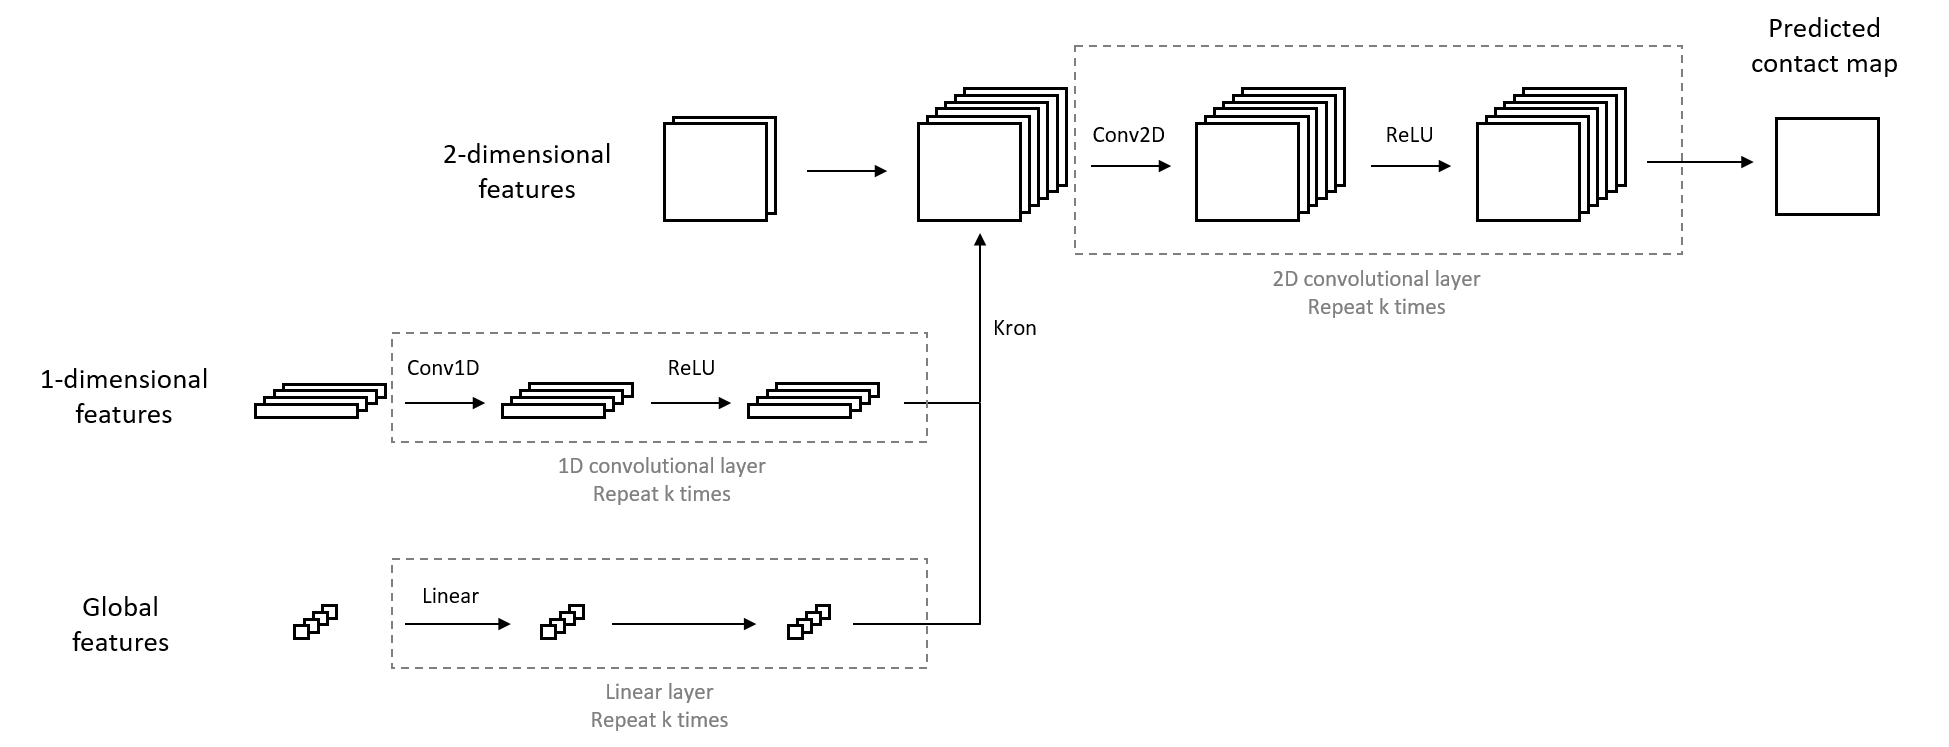
\includegraphics[width=\textwidth, keepaspectratio]{imgs/architecture.png}
       \caption{Proposed architecture of the deep convolutional neural network for semantic segmentation}
      \label{architecture}
    \end{center}
  \end{figure}

\section{Evaluation}

  \subsection{Contact map evaluation}

    Protein contact maps are imbalanced by nature: they contain very few residue contacts compared to their number of residue pairs.
    $L$ being the number of residues in a protein, the number of residue contacts increases linearly with $L$ while the number of residue pairs
    increases quadratically~\cite{OLMEA1997S25}. This is important because one can evaluate a model only on the $L$ (or even less than $L$) predicted
    residue contacts the model is the most confident about. Such evaluation metric is called \textit{best-L/k PPV (Positive Predictive Value)}
    and can be formulated as follows:

    \begin{equation}
      \text{Best-L/k PPV} = \frac{\sum_{\underset {i-j \geq 6}{(i, j) \in B(L/k)}} C_{i, j}}{L/k}
    \end{equation}

    where $C_{i, j} \in \{0, 1\} \ \forall i, j, i-j \ge 6$ are boolean values indicating a predicted contact.
    $B(L/k)$ is the set of $L/k$ residue pairs with most confident (highest) predicted probabilities.
    Contacts under a residue distance of 6 amino acids are not considered during evaludation phase even though they are used during
    training phase.

    Best-L/k PPV can also be split into three separated metrics: short-range, medium-range and long-range contacts.
    These three types of contacts can be defined by the residue separations used by Skwark et al.~\cite{10.1371/journal.pcbi.1003889}:

      \begin{itemize}
        \item Short-range contacts: 6 - 12 residue separation
        \item Medium-range contacts: 12 - 24 residue separation
        \item Long-range contacts: 24+ residue separation
      \end{itemize}

    \subsection{3D model evaluation}

      \todo{TM-score and RMSD}

\section{Hyper-parameter optimization}

  In order to ensure the best hyper-parameters are selected for the model that will be evaluated
  on the benchmark sets, the Hyperopt Python library~\cite{Bergstra_2015} has been used to explore
  the hyper-parameter space and fine-tune the model on the validation set.
  Training and evaluating a deep neural network is very costly and, as a matter of fact,
  each trial point in the hyper-parameter space should be carefully selected. Techniques based
  on grid search do not suit the problem because they are uninformed methods.

  Hyperopt provides an informed search method called Tree-structured Parzen Estimators (TPE)~\cite{bergstra2011algorithms}.
  In Bayesian hyper-optimization, the posterior probability $P(\alpha \vert \mathcal L)$ is defined as a function
  of the hyper-parameter vector $\alpha$ and the loss $\mathcal L$. Contrary to techniques based on Gaussian processes
  that approximates $P(\alpha \vert \mathcal L)$ only, TPE models both posterior $P(\alpha \vert \mathcal L)$ and $P(L)$.
  The prior is iteratively replaced with non-parametric densities based on generated points $\{ \alpha_1, \alpha_2, \dotsc \}$.
  It this search, TPE is an informed search strategy that refines its prior as new points are observed in the
  hyper-parameter space. The "tree structure" is due to the way the posterior is computed.

  Let $f$ be the prediction function of the model (see section \ref{backpropagation} about backpropagation algorithm),
  and let $f(\alpha) \triangleq \text{argmin}_{f(\Theta, \alpha)} \ell \big(f(\Theta, \alpha)\big)$ be the prediction function  % Formalism: meh
  of a trained model that minimizes a given loss function $\ell$ w.r.t. a fixed hyper-parameter vector $\alpha$.
  Let $l(\alpha)$ be the non-parametric density function defined as a mixture of density functions centered each on an
  observation $\{ \alpha^{i} \}$ for which $\mathcal L = c(f(\alpha^{i}))$ is below the threshold $\mathcal L^*$.
  Density function $g(\alpha)$ is defined analogously as a mixture if density functions centered each on one of the
  remaining observations.
  As described in the following equation, the density function to be used to approximate the posterior is
  determined according to whether the threshold $\mathcal L^*$ has been exceeded.

  \begin{equation}
    P(\alpha \vert \mathcal L) =
      \begin{cases}
        l(\alpha) &  \text{if} \, \mathcal L < \mathcal L^* \\
        g(\alpha) &  \text{otherwise}
      \end{cases}
  \end{equation}

  The threshold $\mathcal L^*$ is set as a quantile of the observed values of $\mathcal L$.
  The value to be optimized in TPE is the Expected Improvement (EI), measured as an integral
  of loss improvements weighted by the posterior itself.
  After applying Bayes formule to the posterior, calculus of EI becomes:

  \begin{equation}
    EI_{\mathcal L^*}(\alpha) = \int_{-\infty}^{\mathcal L^*} (\mathcal L^* - \mathcal L) P(\mathcal L \vert \alpha) d\mathcal L
    = \int_{-\infty}^{\mathcal L^*} (\mathcal L^* - \mathcal L) \frac{P(\alpha \vert \mathcal L) P(\mathcal L)}{P(\alpha)} d\mathcal L
  \end{equation}

  In the framework of Adaptive Parzen Estimators, to each hyper-parameter is assigned a prior and a density function,
  and the estimator is built as a weighted mixture of them.
  For example, a continuous variable can be assigned:
  \begin{itemize}
    \item A uniform prior with lower bound $a$ and upper bound $b$.
    \item A function defined as a mixture of Gaussian distributions, each centered on a point of the hyper-parameter
    space. The standard deviation of a particular distribution can be set as the maximum between distances to the left and right
    neighbors.
  \end{itemize}

  The density function is either $l(\alpha)$ or $g(\alpha)$ depending on whether the loss function associated to current
  point is below the threshold or not.

  \begin{table}[H]
    \centering
    \begin{tabular}{|l|c|c|}
      \hline
      Module & Hyper-parameter & Set of values \\
      \hline
      \hline
      General & Batch size & $\{ 1, 2, 4, 8, 16, 32 \}$ \\
              & Batch normalization & $\{ \top, \bot \}$ \\
              & Track running state & $\{ \top, \bot \}$ \\
              & Learning rate & \text{TODO} \\
              & L2 penalty & \text{TODO} \\
              & Parameter optimization & $\{ \text{ADADELTA}, \text{Adagrad}, \text{Adam} \}$ \\
              & Activation function & $\{ \text{ReLU}, \text{ELU}, \text{LeakyReLU}, \text{Tanh} \}$ \\
              & Use global modules & $\{ \top, \bot \}$ \\
      \hline
      Global module & Depth & $\{ 2, 3, 4, 5, 6, 7, 8, 9, 10 \}$ \\
      \hline
      1-dimensional module & Depth & $\{ 2, 3, 4, 5, 6, 7, 8, 9, 10 \}$ \\
                           & Filter size & $\{ 3, 5, 7 \}$ \\
                           & Number of filters & $\{ 8, 16, 32, 64, 128 \}$ \\
      \hline
      2-dimensional module & Depth & $\{ 2, 3, 4, 5, 6, 7, 8, 9, 10 \}$ \\
                           & Filter size & $\{ 3, 5, 7 \}$ \\
                           & Number of filters & $\{ 8, 16, 32, 64, 128 \}$ \\
      \hline
    \end{tabular}
    \captionof{table}{Hyper-parameter space for the proposed architecture.}
    \label{hyperparams}
  \end{table}

\section{Implementation}

  \subsection{Availability}

    Main source code is available at: \,
    \href{https://github.com/AntoinePassemiers/Wynona}{https://github.com/AntoinePassemiers/Wynona}.

    Template-free contact-assisted 3D modelling algorithm is available at: \, \\
    \href{https://github.com/AntoinePassemiers/GDE-GaussFold}{https://github.com/AntoinePassemiers/GDE-GaussFold}.

  \subsection{Deep learning framework}

    Methods and results presented in this thesis have been both implemented and produced in
    Python. The neural architecture has been built on top of PyTorch,
    which is an open source deep learning framework based on Torch~\cite{torch}.

    PyTorch does not natively handle arbitrary-sized inputs, for example fully-convolutional
    neural networks cannot accept images with variable height/width.
    For this aim, it is necessary to add a layer of abstraction so the neural models are
    able to process \textit{virtual batches} of inputs. Let's define a virtual batch as the number
    of samples a model has to process between each parameter update.
    A forward pass on a virtual batch then consists in constructing one computational graph
    per sample and backpropagate the gradients through each one of them separately.
    Once all the gradients have been computed, they are collected and averaged over the sample
    dimension. Pytorch allows to explicitly call the forward pass, backward pass and update
    procedures when needed, which eases the implementation of virtual batch processing.

    Model general architecture is fully-convolutional, forcing us to use only deep learning
    functionalities that are invariant to individual input sizes. These are:

    \begin{itemize}
      \item Element-wise operations like activation functions: ReLU, ELU, Sigmoid, etc.
      \item Dropout, which preserves the dimensionality of its inputs.
      \item Convolution, because convolutional filters have a dimensionality that is
      invariant to the input size (see section \ref{convlayers}).
      \item Batch normalization (see section \ref{batchnorm}).
      \item Many non-neural transformations like arithmetic operations, Einstein
      summation, Kronecker product, etc.
    \end{itemize}

  \subsection{Feature extraction}

    Many features discussed in the present document rely on amino acid counts.
    Despite the fact that counting algorithms such as histograms are embarassingly parallel
    and naturally suitable for multiprocessing, they cannot be efficiently vectorized.
    For this specific reason, the scientific computing library NumPy (which has been extensively
    used during the experiments) is not sufficient to extract this type of features in reasonable
    time. Instead, C extensions have been created using the Cython compiler\cite{behnel2010cython}.

  \subsection{Contact-assisted 3D modelling}

    Contact-assisted 3D modelling algorithm makes use of the Multidimensional scaling algorithm
    as implemented by Scikit-learn~\cite{scikit-learn} and the implementation of Dijkstra's
    algorithm from NetworkX \todo{cite?}.
    Details about the algorithm design are given in appendix.

\todo{Deep architectures in PCP: \cite{di2012deep}}

\section{Hyper-Parameter Optimization}

    \begin{figure}[H]
        \begin{center}
            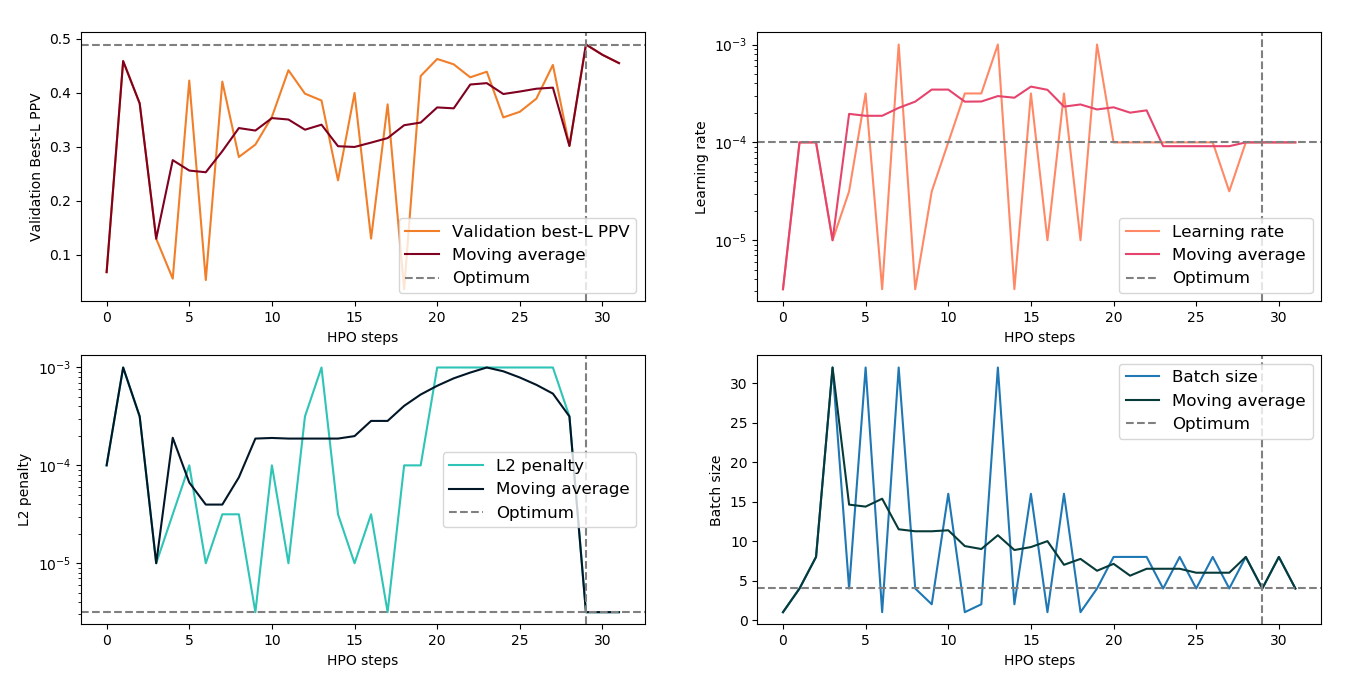
\includegraphics[width=\textwidth, keepaspectratio]{imgs/hpo.png}
            \caption{Performance and hyper-parameter values as a function of the number
            of Hyper-Parameter Optimization (HPO) iterations.
            Top left figure illustrates the optimal point whose value on x-axis
            is given by the HPO iteration that yields highest validation Best-L PPV.
            Optimal values for the learning rate, L2 penalty and batch size are denoted
            by dashed lines in top right, bottom left and bottom right figures, respectively.}
            \label{hpoparams}
        \end{center}
    \end{figure}

    \begin{figure}[H]
        \begin{center}
            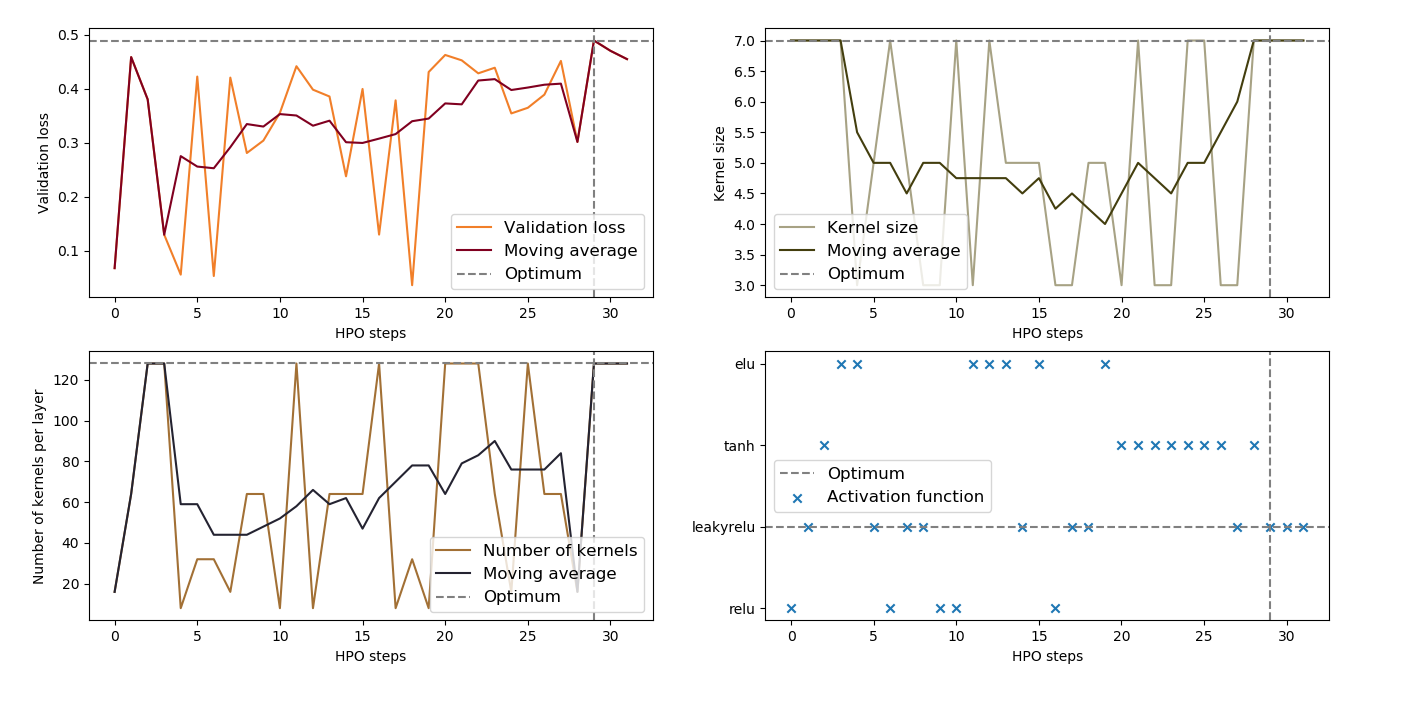
\includegraphics[width=\textwidth, keepaspectratio]{imgs/hpo2.png}
            \caption{Performance and hyper-parameter values as a function of the number
            of Hyper-Parameter Optimization (HPO) iterations.
            Top left figure illustrates the optimal point whose value on x-axis
            is given by the HPO iteration that yields highest validation Best-L PPV.
            Optimal values for kernel size, number of kernels and activation function are denoted
            by dashed lines in top right, bottom left and bottom right figures, respectively.}
            \label{hpoparams2}
        \end{center}
    \end{figure}

    \begin{table}[H]
        \centering
        \begin{tabular}{lll}
          \hline
          Module & Hyper-parameter & Set of values \\
          \hline
          \hline
          General & Batch size & $4$ \\
                  & Batch normalization & $\top$ \\
                  & Track running state & $\bot$ \\
                  & Learning rate & $10^{-4}$ \\
                  & L2 penalty & $10^{-4}$ \\
                  & Parameter optimization & $\text{Adam}$ \\
                  & Activation function & $\text{LeakyReLU}$ \\
                  & Use global modules & $\top$ \\
          \hline
          Global module & Depth & $3$ \\
          \hline
          1-dimensional module & Depth & $18$ \\
                               & Filter size & $7$ \\
                               & Number of filters & $128$ \\
          \hline
          2-dimensional module & Depth & $18$ \\
                               & Filter size & $7$ \\
                               & Number of filters & $128$ \\
          \hline
        \end{tabular}
        \captionof{table}{Set of hyper-parameter values obtained at optimal point.}
        \label{besthp}
    \end{table}

    \begin{figure}[H]
        \begin{center}
            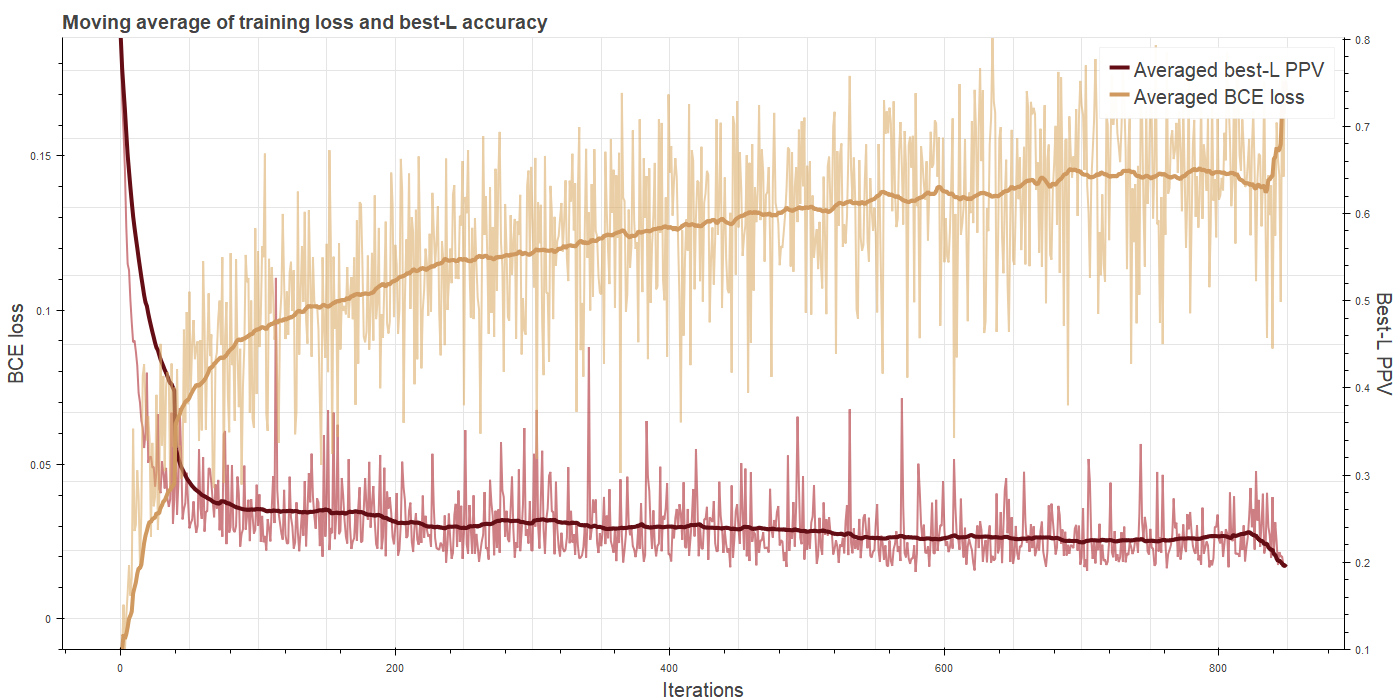
\includegraphics[width=\textwidth, keepaspectratio]{imgs/loss.png}
            \caption{Binary Cross-Entropy loss and best-L PPV computed on
              a rolling window of batches during training phase of the model
              with the best hyper-parameters.}
            \label{lossandppv}
        \end{center}
    \end{figure}

\section{Model evaluation on the different benchmark sets}

    \begin{table}[H]
        \centering
        \resizebox{\textwidth}{!}{
        \begin{tabular}{|l|ccc|ccc|ccc|}
            \hline
            & & CASP11 & & & CAMEO & & & Membrane & \\
            \hline
            Method & Short & Medium & Long & Short & Medium & Long & Short & Medium & Long \\
            \hline
            \hline
            Wynona & 0 & \textbf{0.43} & 0.40 & 0 & \textbf{0.31} & 0.28 & - & - & - \\
            PconsC3 & 0.25 & 0.29 & 0.40 & 0.21 & 0.23 & 0.27 & 0.15 & 0.19 & 0.33 \\
            RaptorX-Contact & \textbf{0.28} & 0.35 & \textbf{0.55} & \textbf{0.23} & 0.28 & \textbf{0.42} & 0.16 & 0.22 & 0.47 \\
            MetaPSICOV & 0.26 & 0.31 & 0.39 & 0.22 & 0.22 & 0.28 & 0.16 & 0.21 & 0.35 \\
            PlmDCA & 0.14 & 0.16 & 0.27 & 0.11 & 0.13 & 0.19 & 0.08 & 0.11 & 0.21 \\
            PSICOV & 0.14 & 0.15 & 0.24 & 0.13 & 0.14 & 0.18 & 0.09 & 0.11 & 0.20 \\
            mfDCA & 0.13 & 0.15 & 0.22 & 0.10 & 0.11 & 0.15 & 0.09 & 0.12 & 0.24 \\
            \hline
        \end{tabular}
        }
        \captionof{table}{Best-L PPV of different methods on short,
        medium and long-range contacts. Results are shown for the three
        different benchmark sets: CASP11 targets, CAMEO proteins, and
        the benchmark set of membrane proteins.}
        \label{benchmark}
    \end{table}

    \subsection{CASP11}

        \todo{}

    \subsection{CAMEO}

        \todo{}

    \subsection{Membrane proteins}

        \todo{}

\section{Sensitivity to the number of homologous sequences}

    \begin{figure}[H]
        \begin{center}
            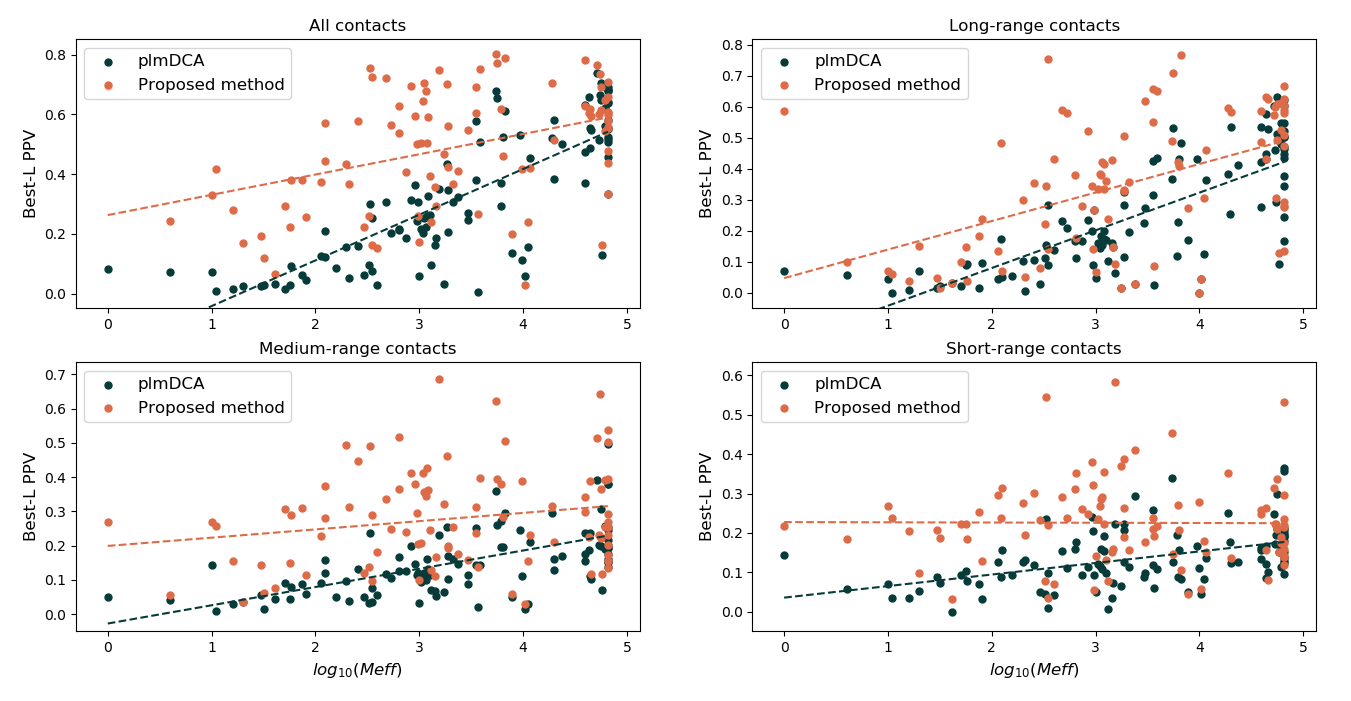
\includegraphics[width=\textwidth, keepaspectratio]{imgs/Meff.png}
            \caption{Performance as a function of the logarithm of the effective
            number of homologous sequences. Top figure shows the results on
            CASP11 targets for all contacts. Bottom left and bottom right figures
            focus on medium-range and long-range contacts, respectively.}
            \label{sensitivity}
        \end{center}
    \end{figure}

\section{Model performance by structural class}

  Automated assignment of CATH C classes: \todo{\cite{michie1996analysis}}

\section{Folding proteins from contact maps}

    \begin{figure}[H]
        \begin{center}
            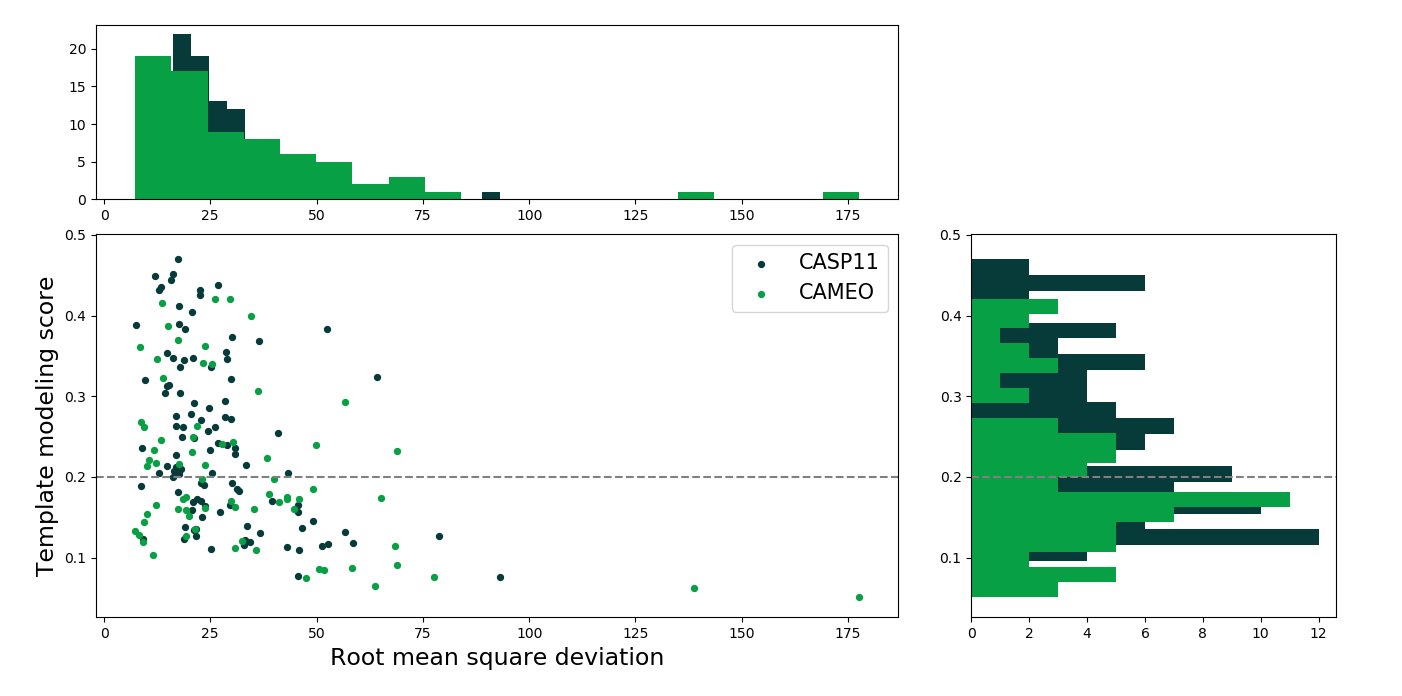
\includegraphics[width=\textwidth, keepaspectratio]{imgs/fold.png}
            \caption{Root mean square deviations and template-modelling scores
            on the 3 benchmark sets.}
            \label{fold}
        \end{center}
    \end{figure}

\todo{tSNE: \cite{Maaten2008VisualizingDU}}

\chapter{Conclusion}


\begin{appendices}
    \chapter{3D model assessment}

    \section{Contact-assisted 3D modelling}

    This appendix describes the algorithm used to reconstruct
    proteins in three dimensions. Like GDFuzz3D~\cite{pietal2015gdfuzz3d},
    it uses graph distances to convert predicted contact maps
    in order to approximate distance maps. However, the proposed method is template-free
    and does not make use of MODELLER~\cite{modeller} as in GDFuzz3D.

    \subsection{Graph distances}

        Let's use the graph representation of contact maps as in section \ref{pcn}
        about Protein Contact Networks.
        The graph distance between two residues is defined as the length of
        the shortest path between them.
        Predicted contact maps are converted to binary adjacency matrices
        by keeping only the $4.5\,L$ top predicted contacts.

    \subsection{Approximate Euclidean distances}

        As explained in \cite{pietal2015gdfuzz3d}, there is a linear relationship
        between graph distances and real euclidean distances.
        Let $GD_{i,j}$ be the graph distance between residues $i$ and $j$. Then
        the euclidean distance $\delta(x_i, x_j)$ between the corresponding
        points $x_i$ and $x_j$ is approximated by:

        \begin{align}
            \delta(x_i, x_j) = 5.72 \times GD_{i,j}
        \end{align}

    \subsection{Gaussian restraints}

        \begin{table}[H]
            \centering
            \begin{tabular}{|l|c|c|c|c|}
                \hline
                Restraint type & Seq. sep. & Graph Distance (GD) & Mean & Standard deviation \\
                \hline
                \hline
                Intra-alpha & 1 & 1 (contact) & 3.82 & 0.35 \\
                Intra-alpha & 2 & 1 (contact) & 5.50 & 0.52 \\
                Intra-alpha & 3 & 1 (contact) & 5.33 & 0.93 \\
                Intra-alpha & 4 & 1 (contact) & 6.42 & 1.04 \\
                Intra-beta  & 1 & 1 (contact) & 3.80 & 0.28 \\
                Intra-beta  & 2 & 1 (contact) & 6.66 & 0.30 \\
                Alpha/beta  & $\ge$ 4 & 1 (contact) & 6.05 & 0.95 \\
                Helix/coil  & $\ge$ 4 & 1 (contact) & 6.60 & 0.92 \\
                Seq. sep.   & $\ge$ 4 & 1 (contact) & 3.82 & 0.39 \\
                All & $\ge$ 4 & any & 5.72 $\times$ GD & 1.34 $\times$ GD \\
                \hline
            \end{tabular}
            \captionof{table}{Gaussian restraints present in the 3D model}
            \label{restraints}
        \end{table}

        The set of points $X$ that best satisfies Gaussian restraints is simply
        obtained by log-likelihood maximization:
        \begin{align}
            \hat{X} & = \text{argmax}_{X} \sum\limits_{i < j ,\, (\mu_{i,j}, \sigma_{i,j}) \in R}
                \Bigg(\frac{\delta(x_i, x_j) - \mu_{i,j}}{\sigma_{i,j}}\Bigg)^2
        \end{align}

    \subsection{Evolutionary algorithm}


\section{Evaluation metrics}

\begin{align}
    \text{TM-score}(X^{(target)}, X^{(aligned)}) = \text{max} \Bigg[ \frac{1}{L} \sum\limits_{i=1}^L 
        \frac{1}{1 + \Big(\frac{\delta(x_i^{(target)}, x_i^{(aligned)})}{\delta_0}\Big)^2} \Bigg]
\end{align}

where $\delta_0 = 1.24 \sqrt[3]{L - 15} - 1.8$.


\begin{align*}
    P(x) & = R^X_{\phi} R^Y_{\psi} R^Z_{\theta} x + b \\
    & =
    \begin{pmatrix}
    1 & 0 & 0 \\
    0 & \cos{\phi} & -\sin{\phi} \\
    0 & \sin{\phi} & \cos{\phi}
    \end{pmatrix}
    \begin{pmatrix}
    \cos{\psi} & 0 & \sin{\psi} \\
    0 & 1 & 0 \\
    -\sin{\psi} & 0 & \cos{\psi}
    \end{pmatrix}
    \begin{pmatrix}
    \cos{\theta} & -\sin{\theta} & 0 \\
    \sin{\theta} & \cos{\theta} & 0 \\
    0 & 0 & 1
    \end{pmatrix}
    x +
    \begin{pmatrix}
    b^X \\
    b^Y \\
    b^Z
    \end{pmatrix}
\end{align*}
\end{appendices}

\appendix

\backmatter

\printindex % use makeindex to generate the index

\bibliographystyle{plain}

\bibliography{report}

\end{document}
